\begin{frame}{Introduction}
\begin{block}{Message passing algorithms}
\begin{itemize}
  \item Remarkably successful in coding theory
  \item Used to design capacity-achieving codes/decoders for a variety of channels
  \item Tools have been developed to analyze their performance
\end{itemize}
\end{block}

\end{frame}
%-------------------------------------------------------
\begin{frame}{Two main goals}
\begin{block}{Goal 1}
 Review some developments in modern coding theory and show how to analyze the performance of a simple peeling decoder for the BEC and $p$-ary symmetric channels.
\end{block}
\pause
\begin{block}{Goal 2}
Show that the following problems have the same structure as channel coding problems and show how to use the \alert{peeling decoder} to solve them.
\end{block}

\begin{block}{Problems}
\begin{itemize}
%\item Rateless codes
\item \alert{Uncoordinated massive multiple access}
\item \alert{Sparse Fourier transform (SFT) computation}
\item Sparse Walsh-Hadamard transform computation	
\item \alert{Compressed sensing}
    \begin{itemize}
    \item Data stream computing
    \item Group testing
    \item Compressive phase retrieval
    \end{itemize}
%\item Sparse covariance estimation
\end{itemize}
\end{block}

%\begin{block}{Outline}
%\begin{itemize}
%  \item Tanner graph representations of codes, LDPC and LDGM ensembles
%  \item Introduce the peeling decoder for BEC
%  \item Analyze the performance of the decoder via density evolution
%  \item Provide a brief overview of how to design optimal code ensembles
%  \item Peeling decoder for the error channel via generalized LDPC/LDGM codes
%  \item Syndrome source coding is the same as error correction
%\end{itemize}
%\end{block}

%\begin{block}{Literature}
%Presented in detail in ``Modern Coding Theory", Richardson and Urbanke
%\end{block}
\end{frame}

%--------------------------------------------------------------------------------------
\begin{frame}{\only<2->{Remembering Sir David MacKay}}
\only<2->{David Mackay's rediscovery of LDPC codes and his very interesting book on Information Theory has undoubtedly had a big influence on the field.}
\begin{columns}
\column{0.5\textwidth}
\includegraphics[width=2.3in]{David_MacKay}
\column{0.5\textwidth}
\only<2->{\includegraphics[width=2.0in]{Mackaybook}}
\end{columns}
\end{frame}
%%--------------------------------------------------------------------------------------
%\begin{frame}{Part II}
%\begin{block}{Goal for Part II}
%Show that the following problems have the same structure as the erasure correction, error correction or syndrome source coding problem and show how to use the \alert{peeling decoder} can be used to solve them
%\end{block}
%
%\begin{block}{Problems}
%\begin{itemize}
%%\item Rateless codes
%\item \alert{Uncoordinated multiple access}
%\item \alert{Sparse Fourier transform (SFT) computation}
%\item Sparse Walsh-Hadamard transform computation	
%\item \alert{Compressed sensing}
%\item Data stream computing
%\item Group testing
%\item Compressive phase retrieval
%\item Sparse covariance estimation
%\end{itemize}
%\end{block}
%
%\end{frame}
%-------------------------------------------------------------
\begin{frame}{Binary erasure channel (BEC) and erasure correction}

\begin{figure}[t]
\centering
\scalebox{0.55}{\input{./Figures/BECsystemmodel.tex}}
\end{figure}

\begin{block}{Channel coding problem}
\begin{itemize}
\item Transmit a message $\underline{m} = [m_1, \ldots, m_k]^T$ through a binary erasure channel
\item Encode the $k$-bit message $\underline{m}$ into a $n$-bit codeword $\underline{x}$
\item Redundancy is measured in terms of rate of the code $R = k/n$
%\item For $p=2$, capacity $C = 1-H_2(\epsilon)$
%\item A sequence of codes $\{\mathcal{C^n}\}$ is capacity achieving if $P_e^n \rightarrow 0$ while the rate $R^n \rightarrow C$
\end{itemize}
\end{block}

\end{frame}

%--------------------------------------------------------------------------------------
\begin{frame}{Binary erasure channel (BEC) and erasure correction}
%\begin{figure}[t]
%\centering
%\includegraphics[width=3.0in]{ParySystemModel}
%\end{figure}
%\vspace*{-5mm}
%\begin{figure}[t]
%\centering
%\includegraphics[width=1.0in,angle=-90]{BECchannelmodel}
%\end{figure}
\vspace*{-3mm}
\begin{figure}[t]
\centering
\scalebox{0.55}{\input{./Figures/BECsystemmodel.tex}}
\end{figure}
\vspace*{-3mm}
\begin{block}{Capacity achieving sequence of codes}
\begin{itemize}
\pause \item Capacity $C(\epsilon) = 1-\epsilon$
\pause  \item A sequence of codes $\{\mathcal{C}^n\}$
  \item Probability of erasure $P_e^n$
  \item Rate $R^n$
  \item Capacity achieving if $P_e^n \rightarrow 0$ as $n \rightarrow \infty$ while $R^n \rightarrow C$
\pause  \item \alert{Find efficient encoders/decoders in terms encoding and decoding complexities}
\end{itemize}
\end{block}
\pause
\begin{block}{Significance of the erasure channel}
\begin{itemize}
  \item Introduced by Elias in 1954 as a toy example
%  \item Good model for transmission of packets over the Internet
  \item Has become the canonical model for coding theorists to gain insight
\end{itemize}
\end{block}


\end{frame}



%%-----------------------------------------------------		
%\begin{frame}{$(n,k)$ Binary linear block codes - basics}
%\begin{block}{Generator matrix - $\mathbf{G}$ is a $n \times k$ encoding matrix}	
%\[
%\begin{bmatrix}
%  g_{1,1} & \cdots & g_{k,l} \\
%  \vdots & \ddots & \vdots \\
%  \vdots & \ddots & \vdots \\
%  g_{n,1} &  & g_{k,l} \\
%\end{bmatrix}
%\begin{bmatrix}
%  m_1 \\
%  \vdots \\
%  m_k \\
%\end{bmatrix}
%=
%\begin{bmatrix}
%  x_1 \\
%  \vdots \\
%  \vdots \\
%  x_n \\
%\end{bmatrix}
%\pause
%\bigoplus
%\begin{bmatrix}
%  e_1 \\
%  \vdots \\
%  \vdots \\
%  e_n \\
%\end{bmatrix}
%=
%\begin{bmatrix}
%  r_1 \\
%  \vdots \\
%  \vdots \\
%  r_n \\
%\end{bmatrix}
%\]
%%\[ \mathbf{G}_{n \times k} \underline{m}_{k \times 1} = \underline{c}_{n \times 1} \oplus \underline{e}_{n \times 1} = \underline{r}_{n \times 1} \]
%\pause
%\begin{eqnarray}
%\nonumber \underline{x} & = & \mathbf{G} \underline{m} \\
%\nonumber \underline{r} & = & \underline{x} \oplus \underline{e}
%\end{eqnarray}
%\end{block}
%\pause
%\begin{block}{Parity check matrix - $\mathbf{H}$ is a $(n-k) \times n$ matrix such that $\mathbf{H} \mathbf{G} = \mathbf{0}$}
%\[
%\underline{y} = \mathbf{H} \underline{r} = \mathbf{H} \underline{x} \oplus \mathbf{H} \underline{e} = \underline{0} \oplus \mathbf{H} \underline{e}
%\]
%\end{block}
%\end{frame}

%-----------------------------------------------------		
\begin{frame}{$(n,k)$ Binary linear block codes - basics}
\begin{columns}[t]
\column{0.47\textwidth}
\begin{block}{$\mathbf{G}$ is a $n \times k$ generator matrix}	
\[
\begin{bmatrix}
  g_{1,1} & \cdots & g_{k,l} \\
  \vdots & \ddots & \vdots \\
  \vdots & \ddots & \vdots \\
  g_{n,1} &  & g_{k,l} \\
\end{bmatrix}
\begin{bmatrix}
  m_1 \\
  \vdots \\
  m_k \\
\end{bmatrix}
=
\begin{bmatrix}
  x_1 \\
  \vdots \\
  \vdots \\
  x_n \\
\end{bmatrix}
\]
\end{block}

\column{0.5\textwidth}
\begin{block}{Example - (6,3) code}
\[
\ \
\begin{bmatrix}
  1 & 0 & 0 \\
  0 & 1 & 0 \\
  0 & 0 & 1 \\
  1 & 0 & 1 \\
  1 & 1 & 0 \\
  0 & 1 & 1 \\
\end{bmatrix}
\begin{bmatrix}
  1 \\
  1 \\
  0 \\
\end{bmatrix}
=
\begin{bmatrix}
1\\
1\\
0\\
1\\
0\\
1\\
\end{bmatrix}
\]
\end{block}
\end{columns}
\pause
\begin{block}{Parity check matrix - $\mathbf{H}$ is a $(n-k) \times n$ matrix s.t. $\Hm \Gm = \mathbf{0} \Rightarrow \Hm \xv = 0$}
\[
\Hm = \begin{bmatrix}
  1 & 0 & 1 & 1 & 0 & 0 \\
  1 & 1 & 0 & 0 & 1 & 0 \\
  0 & 0 & 1 & 0 & 0 & 1 \\
\end{bmatrix}
\begin{bmatrix}
1\\
1\\
0\\
1\\
0\\
1\\
\end{bmatrix}
=
\begin{bmatrix}
0\\
0\\
0\\
\end{bmatrix}
\]
\end{block}
\end{frame}

%%--------------------------------------------------------------------------------------
%\begin{frame}{Brief survey of the literature}
%\begin{itemize}
%\item The binary erasure channel (BEC) introduced by Elias in 1954
%\pause
%\item Regular LDPC codes introduced by Gallager in 1962, 1963
%\pause
%\item Zyablov and Pinsker considered peeling decoder in 1974
%\pause
%\item Papers by Luby, Mitzenmacher, Shokrollahi, Spielman, Stemann 1997-2001
%\pause
%\item Rateless codes introduced by Luby in 2002
%\pause
%\item EXIT chart analysis by ten Brink'99 and Ashikmin, Kramer and ten Brink'04
%\pause
%\item Summarized in Modern coding theory book by Richardson and Urbanke
%\end{itemize}
%\end{frame}
%--------------------------------------------------------------------------------------
\begin{frame}{Tanner graph representation of codes}
\begin{columns}
\column{0.5\textwidth}
\includegraphics[width=2.3in,angle=-90]{paritycheckmatrix63code}
\column{0.5\textwidth}
\includegraphics[width=2.25in,angle=-90]{Tannergraph63code}
\end{columns}
\begin{block}{}
\begin{itemize}
    \item Gallager'63, Tanner'81
    \item Parity check matrix implies that $\Hm \xv = 0$
    \item Code constraints can be specified in terms of a bipartite (Tanner) graph
  %\item A code can be specified by giving the Tanner graph
\end{itemize}
\end{block}
\end{frame}
%--------------------------------------------------------------------------------------
\begin{frame}{Peeling decoder for the BEC}
\vspace{-5mm}
\begin{columns}
\column{0.5\textwidth}
\includegraphics[width=2.3in,angle=-90]{paritycheckmatrix63code}
\column{0.5\textwidth}
%\includegraphics[width=2.25in,angle=-90]{Tannergraph63codewitherasures}
\scalebox{1}{\pgfdeclarelayer{background}
\pgfdeclarelayer{foreground}
\pgfdeclarelayer{m-f}
\pgfdeclarelayer{main}

\pgfsetlayers{background,foreground}
\colorlet{LightBlue}{blue!10!white}
\colorlet{DarkBlue}{blue!80!white}

\begin{tikzpicture}[scale=1.0]
\clip (-0.15in,0.15in) rectangle (1.3in,-2.5in);

\def\n     {6}   % #-Variable nodes
\def\m     {3}  % #-Check nodes
\def\nodewidth{0.15in}
\def\nodegapVN{0.3in}
\def\nodegapCN{0.5in}

\tikzstyle{check} = [rectangle, draw, text centered, thick, fill=red,
                          minimum height=\nodewidth, minimum width=\nodewidth]
\tikzstyle{bit} = [circle, draw, text centered, thick, fill=LightBlue,
                          radius=0.5*\nodewidth]
\tikzstyle{bitpeeled} = [circle, draw, text centered, thick, fill=DarkBlue,
                          radius=0.5*\nodewidth]

\begin{pgfonlayer}{background}
%\draw[gray,step=0.5in] (-0.15in,0.15in) grid (1.5in,-2.5in);
\foreach \vn in {1,...,\n}{
  \node[bit] (vn\vn) at (0,-\vn*\nodegapVN) {};
 }

 \foreach \cn in {1,...,\m}{
  \node[check] (cn\cn) at (1in,-\cn*\nodegapCN) {};
 }
\end{pgfonlayer}



\begin{pgfonlayer}{foreground}

%Text to left of VN
\only<1>{
\foreach \vn in {1,...,\n}{
  \node[left] (nodetxt) at (vn\vn.west) {\normalsize{$x_\vn$}};
 	}  	
}

\only<2-8>{
\foreach \vn/\txt in {2/1,4/1,5/0}{
\node[left] (nodetxt) at (vn\vn.west) {\normalsize{\txt}};
 	}	
}

\only<2-3>\node[left] (nodetxt) at (vn1.west) {\normalsize{E}};
\only<2-5>\node[left] (nodetxt) at (vn3.west) {\normalsize{E}};
\only<2-7>\node[left] (nodetxt) at (vn6.west) {\normalsize{E}};


\only<4-8>\node[left] (nodetxt) at (vn1.west) {\normalsize{E=1}};
\only<6-8>\node[left] (nodetxt) at (vn3.west) {\normalsize{E=0}};
\only<8>\node[left] (nodetxt) at (vn6.west) {\normalsize{E=1}};

%Edges
\uncover<1-2>{
\foreach \vn/\cn in {2/2,2/3,4/1,5/2}{
 \draw[thick] (vn\vn.east)--(cn\cn.west);
  }
}

\only<1-3>\draw[thick] (vn1.east)--(cn2.west);
\only<1-4>\draw[thick] (vn1.east)--(cn1.west);

\only<1-5>\draw[thick] (vn3.east)--(cn1.west);
\only<1-6>\draw[thick] (vn3.east)--(cn3.west);

\only<1-5>\draw[thick] (vn3.east)--(cn1.west);
\only<1-6>\draw[thick] (vn3.east)--(cn3.west);

\only<1-7> \draw[thick] (vn6.east)--(cn3.west);

%% Peeled bits color
\uncover<3-8>{
  \foreach \vn in {2,4,5}{
    \node[bitpeeled] () at (vn\vn) {};
    }
  }
 \only<4-8>\node[bitpeeled] () at (vn1) {};
 \only<6-8>\node[bitpeeled] () at (vn3) {};
  \only<8>\node[bitpeeled] () at (vn6) {};

%Check node values
\only<2,5,6,7,8> \node[right] (nodetxt) at (cn1.east) {\normalsize{0}};
\only<3,4> \node[right] (nodetxt) at (cn1.east) {\normalsize{1}};

\only<2,4,5,6,7,8> \node[right] (nodetxt) at (cn2.east) {\normalsize{0}};
\only<3> \node[right] (nodetxt) at (cn2.east) {\normalsize{1}};

\only<2,6,7,8> \node[right] (nodetxt) at (cn3.east) {\normalsize{0}};
\only<3,4,5> \node[right] (nodetxt) at (cn3.east) {\normalsize{1}};



%% Text at the bottom
\only<1> \node[minimum width=10cm] (txt) at (0.5in,-7*\nodegapVN) {Tanner Graph};
\only<2> \node[minimum width=10cm] (txt) at (0.5in,-7*\nodegapVN) {Received block};
\only<3> \node[minimum width=10cm] (txt) at (0.5in,-7*\nodegapVN) {Peeling Step 1};
\only<4-5> \node[minimum width=10cm] (txt) at (0.5in,-7*\nodegapVN) {Peeling Step 2};
\only<6-7> \node[minimum width=10cm] (txt) at (0.5in,-7*\nodegapVN) {Peeling Step 3};
\only<8> \node[minimum width=10cm] (txt) at (0.5in,-7*\nodegapVN) {Peeling Step 4};

\end{pgfonlayer}
\end{tikzpicture} }
\end{columns}
\begin{block}{}
\begin{itemize}
  \item Zyablov and Pinsker'74, Luby et al '95
  \item Remove edges incident on known variable nodes and adjust check node values
  \item If there is a check node with a \alert{single edge}, it can be recovered
\end{itemize}
\end{block}
\end{frame}
%--------------------------------------------------------------------------------------
\begin{frame}{Message passing decoder for the BEC}
\vspace{-5mm}
\begin{columns}
\column{0.5\textwidth}
%\includegraphics[width=2.3in,angle=-90]{paritycheckmatrix63code}
%\includegraphics[width=2.25in,angle=-90]{Tannergraph63codewitherasures}
\scalebox{1}{\pgfdeclarelayer{background}
\pgfdeclarelayer{foreground}
\pgfdeclarelayer{m-f}
\pgfdeclarelayer{main}

\pgfsetlayers{background,foreground}
\colorlet{LightBlue}{blue!10!white}
\colorlet{DarkBlue}{blue!80!white}

\begin{tikzpicture}[scale=1.0]
\clip (-0.15in,0.15in) rectangle (1.3in,-2.5in);

\def\n     {6}   % #-Variable nodes
\def\m     {3}  % #-Check nodes
\def\nodewidth{0.15in}
\def\nodegapVN{0.3in}
\def\nodegapCN{0.5in}

\tikzstyle{check} = [rectangle, draw, text centered, thick, fill=red,
                          minimum height=\nodewidth, minimum width=\nodewidth]
\tikzstyle{bit} = [circle, draw, text centered, thick, fill=LightBlue,
                          radius=0.5*\nodewidth]
\tikzstyle{bitpeeled} = [circle, draw, text centered, thick, fill=DarkBlue,
                          radius=0.5*\nodewidth]

\begin{pgfonlayer}{background}
%\draw[gray,step=0.5in] (-0.15in,0.15in) grid (1.5in,-2.5in);
\foreach \vn in {1,...,\n}{
  \node[bit] (vn\vn) at (0,-\vn*\nodegapVN) {};
 }

 \foreach \cn in {1,...,\m}{
  \node[check] (cn\cn) at (1in,-\cn*\nodegapCN) {};
 }
\end{pgfonlayer}



\begin{pgfonlayer}{foreground}

%Text to left of VN
\only<1>{
\foreach \vn in {1,...,\n}{
  \node[left] (nodetxt) at (vn\vn.west) {\normalsize{$x_\vn$}};
 	}  	
}

\only<2-8>{
\foreach \vn/\txt in {2/1,4/1,5/0}{
\node[left] (nodetxt) at (vn\vn.west) {\normalsize{\txt}};
 	}	
}

\only<2-3>\node[left] (nodetxt) at (vn1.west) {\normalsize{E}};
\only<2-5>\node[left] (nodetxt) at (vn3.west) {\normalsize{E}};
\only<2-7>\node[left] (nodetxt) at (vn6.west) {\normalsize{E}};


\only<4-8>\node[left] (nodetxt) at (vn1.west) {\normalsize{E=1}};
\only<6-8>\node[left] (nodetxt) at (vn3.west) {\normalsize{E=0}};
\only<8>\node[left] (nodetxt) at (vn6.west) {\normalsize{E=1}};

%Edges
\uncover<1-2>{
\foreach \vn/\cn in {2/2,2/3,4/1,5/2}{
 \draw[thick] (vn\vn.east)--(cn\cn.west);
  }
}

\only<1-3>\draw[thick] (vn1.east)--(cn2.west);
\only<1-4>\draw[thick] (vn1.east)--(cn1.west);

\only<1-5>\draw[thick] (vn3.east)--(cn1.west);
\only<1-6>\draw[thick] (vn3.east)--(cn3.west);

\only<1-5>\draw[thick] (vn3.east)--(cn1.west);
\only<1-6>\draw[thick] (vn3.east)--(cn3.west);

\only<1-7> \draw[thick] (vn6.east)--(cn3.west);

%% Peeled bits color
\uncover<3-8>{
  \foreach \vn in {2,4,5}{
    \node[bitpeeled] () at (vn\vn) {};
    }
  }
 \only<4-8>\node[bitpeeled] () at (vn1) {};
 \only<6-8>\node[bitpeeled] () at (vn3) {};
  \only<8>\node[bitpeeled] () at (vn6) {};

%Check node values
\only<2,5,6,7,8> \node[right] (nodetxt) at (cn1.east) {\normalsize{0}};
\only<3,4> \node[right] (nodetxt) at (cn1.east) {\normalsize{1}};

\only<2,4,5,6,7,8> \node[right] (nodetxt) at (cn2.east) {\normalsize{0}};
\only<3> \node[right] (nodetxt) at (cn2.east) {\normalsize{1}};

\only<2,6,7,8> \node[right] (nodetxt) at (cn3.east) {\normalsize{0}};
\only<3,4,5> \node[right] (nodetxt) at (cn3.east) {\normalsize{1}};



%% Text at the bottom
\only<1> \node[minimum width=10cm] (txt) at (0.5in,-7*\nodegapVN) {Tanner Graph};
\only<2> \node[minimum width=10cm] (txt) at (0.5in,-7*\nodegapVN) {Received block};
\only<3> \node[minimum width=10cm] (txt) at (0.5in,-7*\nodegapVN) {Peeling Step 1};
\only<4-5> \node[minimum width=10cm] (txt) at (0.5in,-7*\nodegapVN) {Peeling Step 2};
\only<6-7> \node[minimum width=10cm] (txt) at (0.5in,-7*\nodegapVN) {Peeling Step 3};
\only<8> \node[minimum width=10cm] (txt) at (0.5in,-7*\nodegapVN) {Peeling Step 4};

\end{pgfonlayer}
\end{tikzpicture} }
\column{0.5\textwidth}
\includegraphics[width=2.25in,angle=-90]{Tannergraph63codewitherasures}
\end{columns}
\vspace{-5mm}
\begin{block}{}
\begin{itemize}
  \item Pass messages between variable nodes and check nodes along the edges
  \item Messages $\in \{\text{value of var node (NE), erasure (E)}\}$
  \item Var-to-check node message is NE if \alert{at least one incoming message is NE}
  \item Check-to-var node message is NE if \alert{all other incoming messages are NE}
\end{itemize}
\end{block}
\end{frame}
%--------------------------------------------------------------------------------------
\begin{frame}{Peeling decoder is a greedy decoder}
\vspace{-3mm}
\begin{columns}
\column{0.5\textwidth}
\[
\Hm = \begin{bmatrix}
      x_1 & x_2 & x_3 & x_4 & x_5 & x_6 \\
      1 & 1 & 1 & 1 & 0 & 0 \\
      1 & 1 & 0 & 0 & 1 & 0 \\
      0 & 1 & 1 & 0 & 0 & 1 \\
    \end{bmatrix}
\]
\begin{eqnarray*}
% \nonumber % Remove numbering (before each equation)
  x_1 \oplus x_2 \oplus x_3 \oplus x_4 &=& 0 \\
  x_1 \oplus x_2 \oplus x_5 &=& 0 \\
  x_2 \oplus x_3 \oplus x_6 &=& 0
\end{eqnarray*}
\column{0.5\textwidth}
\includegraphics[width=2.25in,angle=-90]{Tannergraph63codestoppingset}
\end{columns}
\pause
\vspace{-3mm}
\begin{columns}
\column{0.5\textwidth}
\begin{block}{Linearly independent set of equations}
\begin{eqnarray*}
% \nonumber % Remove numbering (before each equation)
  x_1 \oplus x_2 \oplus x_3 & = & x_4 \\
  x_1 \oplus x_2  &=& x_5 \\
  x_2 \oplus x_3  &=& x_6
\end{eqnarray*}
\end{block}
\column{0.5\textwidth}
\end{columns}
\end{frame}
%--------------------------------------------------------------------------------------
\begin{frame}{Degree distributions}
\begin{columns}
\begin{column}{0.43\textwidth}
\begin{center}
\includegraphics[width=2.0in,angle=-90]{Tannergraph63codestoppingset}
\end{center}
\end{column}
\begin{column}{0.57\textwidth}
\only<5>{
\begin{itemize}
%\item $L(x) = \frac{3}{6} x + \frac26 x^2 + \frac16 x^3$
%\vspace{3mm}
%\item $\lambda(x) = \frac{3}{10} + \frac{4}{10} x + \frac {3}{10} x^2$
%\vspace{3mm}
%\item $R(x) = \frac{2}{3}x^3 + \frac13 x^4$
%\vspace{3mm}
%\item $\rho(x) = \frac{6}{10} x^2+ \frac{4}{10} x^3$
%\item $l_{\text{avg}} = L'(1) = \frac{1}{\int_{0}^{1} \lambda(x) \ dx}$
%\item $r_{\text{avg}} = R'(1) = \frac{1}{\int_{0}^{1} \rho(x) \ dx}$
\item Rate - $r(\lambda,\rho) = 1-\frac{{l_{\text{avg}}}}{{r_{\text{avg}}}} = 1 - \frac{\int_{0}^{1} \rho(x) \ dx}{\int_{0}^{1} \lambda(x) \ dx}$
\end{itemize}
}
\end{column}
\end{columns}

\begin{itemize}
\item VN d.d. from node perspective - $L(x) = \sum_i L_i x^i = \frac{3}{6} x + \frac26 x^2 + \frac16 x^3$
\vspace{1mm}
\pause
\item VN d.d. from edge perspective - $\lambda(x) = \sum_i \lambda_i x^{i-1} = \frac{3}{10} + \frac{4}{10} x + \frac {3}{10} x^2$
\vspace{1mm}
\pause
\item CN d.d. from node perspective - $R(x) = \sum_i R_i x^i = \frac{2}{3}x^3 + \frac13 x^4 $
\vspace{1mm}
\pause
\item CN d.d. from edge perspective - $\rho(x) =\sum_i \rho_i x^{i-1} = \frac{6}{10} x^2+ \frac{4}{10} x^3$
\end{itemize}

\end{frame}
%--------------------------------------------------------------------------------------
\begin{frame}{LDPC code ensemble}
\begin{center}
  %\scalebox{1}{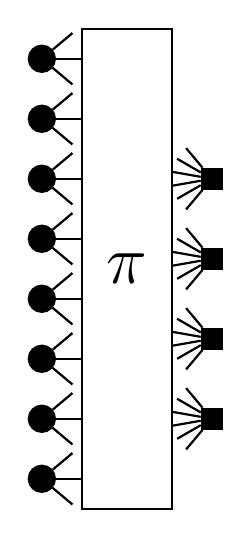
\begin{tikzpicture}
\def\horzgap{0.85in}; %Horizontal gap between nodes/levels
\def \gapVN{0.3in}; %vertical gap between nodes
\def \gapCN{0.4in}; %Horizontal gap between nodes

\def \textoffs{0.12in}; %Offset for writing text above a node
\def\nodewidth{0.1in};
\def\ext{0.2in};

\def \n {8};
\def\ldeg{3};
\def \m {4};
\def\rdeg{6};
\def\langle{40};%120 degrees/3
\def\langle{20};%120 degrees/6

\tikzstyle{check} = [rectangle, draw, text centered, thick, fill=black,
                          minimum height=\nodewidth, minimum width=\nodewidth]
\tikzstyle{bit} = [circle, draw, text centered, thick,fill=black,
                          radius=0.5*\nodewidth]
                          
\foreach \vn in {1,...,\n}{
 \node[bit] (vn\vn) at (0,\vn*\gapVN) {};
  \draw[thick] (vn\vn) --+ (+40:\ext); 
  \draw[thick] (vn\vn ) --+ (0:\ext); 
   \draw[thick] (vn\vn ) --+ (-40:\ext); 
}

\foreach \cn in {1,...,\m}{
\node[check] (cn\cn) at (\horzgap,0.2in+\cn*\gapCN) {};

 \draw[thick] (cn\cn ) --+ (+130:\ext); 
 \draw[thick] (cn\cn ) --+ (+150:\ext); 
 \draw[thick] (cn\cn ) --+ (+170:\ext); 
 \draw[thick] (cn\cn ) --+ (+190:\ext); 
 \draw [thick](cn\cn ) --+ (+210:\ext); 
 \draw [thick](cn\cn) --+ (+230:\ext); 

% \draw[thick] (cn\cn.west ) --+ (+130:\ext); 
% \draw[thick] (cn\cn.west ) --+ (+150:\ext); 
% \draw[thick] (cn\cn.west ) --+ (+170:\ext); 
% \draw[thick] (cn\cn.west ) --+ (+190:\ext); 
% \draw [thick](cn\cn.west ) --+ (+210:\ext); 
% \draw [thick](cn\cn.west) --+ (+230:\ext); 
}
\node[draw,minimum width=\horzgap-2*\ext,minimum height=\n*\gapVN,thick]() at (0.5*\horzgap,4.5*\gapVN){\Huge{$\pi$}};

\end{tikzpicture}}
\includegraphics[width=2.2in]{LDPCensemble}
\end{center}
\vspace*{-3mm}
\begin{block}{LDPC($n,\lambda,\rho$) ensemble}
\begin{itemize}
\item Ensemble of codes obtained by using different permutations $\pi$
\item Assume there is only one edge between every var node and check node
\item For every $n$, we get an ensemble of codes with the same $(\lambda,\rho)$
%\item Almost all codes in the ensemble have the same rate
\item \alert{Low density parity check} (LDPC) ensemble if graph is of low density
\end{itemize}
\end{block}
\end{frame}
%%--------------------------------------------------------------------------------------
%\begin{frame}{Rate of the code (ensemble)}
%\begin{itemize}
%  \item $l_{\text{avg}} = L'(1) = \frac{1}{\int_{0}^{1} \lambda(x) \ dx}$
%  \item $r_{\text{avg}} = R'(1) = \frac{1}{\int_{0}^{1} \rho(x) \ dx}$
%  \item Rate $\boxed{r(\lambda,\rho) = 1-\frac{{l_{\text{avg}}}}{{r_{\text{avg}}}} = 1 - \frac{\int_{0}^{1} \rho(x) \ dx}{\int_{0}^{1} \lambda(x) \ dx}}$
%\end{itemize}
%\end{frame}
%--------------------------------------------------------------------------------------
\begin{frame}{Analysis of the message passing decoder}
\begin{block}{}
\begin{itemize}
  \item If we pick a code uniformly at random from the LDPC$(n,\lambda,\rho)$ ensemble and use it over a BEC($\epsilon$) with $l$ iterations of message passing decoding, what will be the probability of erasure $P_{e}^n$ in the limit $l,n \rightarrow \infty$ ?
      \pause
    \begin{itemize}
      \item Analyze the average prob. of erasure over the ensemble
      \item For almost all realizations $P_{e}^n$ concentrates around the average
    \end{itemize}
\end{itemize}
\end{block}
\pause
\begin{block}{Relevant literature}
\begin{itemize}
    \item Papers by Luby, Mitzenmacher, Shokrollahi, Spielman, Stemann 97-'02
    \item Explained in Modern coding theory by Richardson and Urbanke
    \item Henry Pfister's course notes on his webpage
\end{itemize}
\end{block}
\end{frame}
%--------------------------------------------------------------------------------------
\begin{frame}{Analysis of the message passing decoder}
\begin{block}{Computation graph}
Computation graph $\mathcal{C}_{l}(x_1,\lambda,\rho)$ of bit $x_{1}$ of depth $l$ ($l$-iterations) is the neighborhood graph of node $x_1$ of radius $l$. \pause Consider the example $\mathcal{C}_{l=1}(\lambda(x)=x,\rho(x)=x^2)$
\end{block}

\begin{columns}
\begin{column}{0.33\textwidth}
\begin{center}
\scalebox{0.6}{\input{./Figures/compGraph1.tex}}
%$G_1$\\$Pr(\mathcal{C}_l(x_1)=G_1)=
\\$1-O(1/n)$
\end{center}
\end{column}

\begin{column}{0.33\textwidth}
\begin{center}
\scalebox{0.6}{
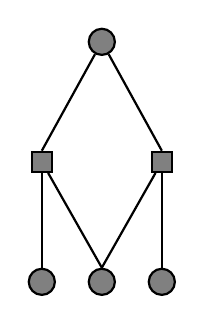
\begin{tikzpicture}
\def \depth{0.6in}; %vertical gap between nodes/levels
\def \gap{0.3in}; %Horizontal gap between nodes
\def \gapA{0.15in}; %Encoder Width
\def \textoffs{0.12in}; %Offset for writing text above a node
\def\nodewidth{0.1in};
\tikzstyle{check} = [rectangle, draw, text centered, thick, fill=gray,
                          minimum height=\nodewidth, minimum width=\nodewidth]
\tikzstyle{bit} = [circle, draw, text centered, thick, fill=gray,
                          radius=0.5*\nodewidth]
                          
\def \fsize{\normalsize}; %Defining a generic font size to be adjusted depending on the scaling
\def \dotsize{\Huge}; %Defining a generic font size to be adjusted depending on the scaling


\node [bit](b1) at (0,0) {} ;

%Level 2
\node[check] (c21) at ([xshift=-\gap,yshift=-\depth]b1) {};
\node[check] (c22) at ([xshift=+\gap,yshift=-\depth]b1) {};

%Lines form level 1-level 2
\draw[thick](b1)--(c21.north);
\draw[thick](b1)--(c22.north);

%Level 3
\node[bit] (b31) at ([xshift=0,yshift=-\depth]c21) {};
\node[bit] (b32) at ([xshift=+\gap,yshift=-\depth]c21) {};
\node[bit] (b33) at ([xshift=0,yshift=-\depth]c22) {};

%Lines form level 2-level 3
\draw[thick](c21)--(b31.north);
\draw[thick](c21)--(b32.north);
\draw[thick](c22)--(b33.north);
\draw[thick](c22)--(b32.north);

\end{tikzpicture}}
%$G_2$\\ \scriptsize{$Pr(\mathcal{C}_l(x_1)=G_2)=O(1/n)$}
\\$O(1/n)$
\end{center}
\end{column}

\begin{column}{0.33\textwidth}
\begin{center}
\scalebox{0.6}{\input{./Figures/compGraph3.tex}}
%$G_3$\\ $Pr(\mathcal{C}_l(x_1)=G_3)=O(1/n^2)$
\\$O(1/n^2)$
\end{center}
\end{column}

\end{columns}
\pause
\begin{block}{Computation tree}
For fixed $(l_{max},r_{max})$, in the limit of large block lengths a computation graph of depth-$l$ looks like a tree with high probability
\end{block}
\end{frame}
%--------------------------------------------------------------------------------------
\begin{frame}{Analysis of the message passing decoder}

\begin{block}{Computation Tree Ensemble-$\mathcal{T}_{l}(\lambda,\rho)$}
Ensemble of bipartite trees of depth $l$ rooted in a variable node (VN) where
\begin{itemize}
\item Root node has $i$ children(CN's) with probability $L_i$
\item Each VN has $i$ children(CN's) with probability $\lambda_i$
\item Each CN has $i$ children(VN's) with probability $\rho_i$
\end{itemize}
\end{block}

\begin{block}{Example: $\mathcal{C}_{l=1}(\lambda(x)=x,\rho(x)=x^2)$}
\begin{center}
\scalebox{0.6}{\input{./Figures/compGraph1.tex}}
\end{center}
\end{block}

\end{frame}
%---------------------------------------------------------------------------------------------------------------------------
\begin{frame}{Density evolution}
\begin{columns}
\begin{column}{0.65\textwidth}
\begin{centering}
\scalebox{0.73}{\begin{tikzpicture}
\def \depth{0.8in}; %Encoder Length
\def \gap{1in}; %Encoder Width
\def \gapA{0.2in}; %Encoder Width
\def\nodewidth{0.1in};
\tikzstyle{check} = [rectangle, draw, text centered, thick,fill=gray,
                          minimum height=\nodewidth, minimum width=\nodewidth]
\tikzstyle{bit} = [circle, draw, text centered, thick,fill=gray,
                          radius=0.5*\nodewidth]

\def \fsize{\normalsize}; %Defining a generic font size to be adjusted depending on the scaling
\def \dotsize{\Huge}; %Defining a generic font size to be adjusted depending on the scaling

\node [bit](b1) at (0,0) {} ;
%\node() at ([yshift=0.12in]b1) {$x_{\text{DE}}^{(l)}=\epsilon \sum_{i} \lambda y_l^{i-1}$ };

%Level 2
\node[check] (c21) at ([xshift=-\gap,yshift=-\depth]b1) {};
\node[check] (c22) at ([yshift=-\depth]b1) {};
\node[check] (c23) at ([xshift=+\gap,yshift=-\depth]b1) {};

%Lines form level 1-level 2
\begin{scope}[thick,decoration={
    markings,
    mark=at position 0.5 with {\arrow{>}}}
    ]
\draw[postaction={decorate}] (b1)--+(0,+0.2in)node[midway,right]{$x_{l}=\epsilon \sum_{i} \lambda_i y_l^{i-1} = \epsilon \lambda(y_l)$ };
\draw[postaction={decorate}](c21.north)--(b1);
\draw[postaction={decorate}](c22)--(b1);
\draw[postaction={decorate}](c23.north)--(b1)node[midway,right]{$y_{l}=1-\rho(1- x_{l-1})$};
\end{scope}

%Level 3
\node[bit] (b31) at ([xshift=-2*\gapA,yshift=-\depth]c21) {};
\node[bit] (b32) at ([xshift=-\gapA,yshift=-\depth]c21) {};
\node[bit] (b33) at ([yshift=-\depth]c21) {};
\node[bit] (b34) at ([xshift=+\gapA,yshift=-\depth]c21) {};
\node[bit] (b35) at ([xshift=2*\gapA,yshift=-\depth]c21) {};

\node[bit] (b36) at ([xshift=-2*\gapA,yshift=-\depth]c22) {};
\node[bit] (b37) at ([xshift=-\gapA,yshift=-\depth]c22) {};
\node[bit] (b38) at ([yshift=-\depth]c22) {};
\node[bit] (b39) at ([xshift=+\gapA,yshift=-\depth]c22) {};
\node[bit] (b310) at ([xshift=2*\gapA,yshift=-\depth]c22) {};

\node[bit] (b311) at ([xshift=-2*\gapA,yshift=-\depth]c23) {};
\node[bit] (b312) at ([xshift=-\gapA,yshift=-\depth]c23) {};
\node[bit] (b313) at ([yshift=-\depth]c23) {};
\node[bit] (b314) at ([xshift=+\gapA,yshift=-\depth]c23) {};
\node[bit] (b315) at ([xshift=2*\gapA,yshift=-\depth]c23) {};


%Lines form level 2-level 3
\begin{scope}[thick,decoration={
    markings,
    mark=at position 0.5 with {\arrow{<}}}
    ]
\draw[postaction={decorate}](c21)--(b31.north);
\draw[postaction={decorate}](c21)--(b32.north);
\draw[postaction={decorate}](c21)--(b33.north);
\draw[postaction={decorate}](c21)--(b34.north);
\draw[postaction={decorate}](c21)--(b35.north);

\draw[postaction={decorate}](c22)--(b36.north);
\draw[postaction={decorate}](c22)--(b37.north);
\draw[postaction={decorate}](c22)--(b38.north);
\draw[postaction={decorate}](c22)--(b39.north);
\draw[postaction={decorate}](c22)--(b310.north);

\draw[postaction={decorate}](c23)--(b311.north);
\draw[postaction={decorate}](c23)--(b312.north);
\draw[postaction={decorate}](c23)--(b313.north);
\draw[postaction={decorate}](c23)--(b314.north);
\draw[postaction={decorate}](c23)--(b315.north)node[midway,right]{$x_{l-1}$};%=\epsilon \sum_i \lmb_i y_l^{i-1}  $};
\end{scope}


\node(brace11) at ([xshift=-0.6in]c21.north){};
\node(brace12) at ([xshift=-0.6in]b33.south){};
\draw [decorate,thick,decoration={brace,amplitude=4pt,mirror}](brace11) -- (brace12) node [black,midway,left,xshift=-5pt]{\fsize Depth-$1$};

 \node (dots1) at ([yshift=-0.4*\depth]b38){\dotsize $\vdots$};
\node (dots2) at ([yshift=-0.6*\depth]b38){\dotsize $\vdots$};


%Lines form level 3-level 4
\def \offsx{0.05in};
\def \offsy{0.1in};
\draw[->,thick](b31.south)+(-\offsx,-\offsy)--(b31.south); \draw[->,thick](b31.south)+(\offsx,-\offsy)--(b31.south);
\draw[->,thick](b32.south)+(-\offsx,-\offsy)--(b32.south); \draw[->,thick](b32.south)+(\offsx,-\offsy)--(b32.south);
\draw[->,thick](b33.south)+(-\offsx,-\offsy)--(b33.south); \draw[->,thick](b33.south)+(\offsx,-\offsy)--(b33.south);
\draw[->,thick](b34.south)+(-\offsx,-\offsy)--(b34.south); \draw[->,thick](b34.south)+(\offsx,-\offsy)--(b34.south);
\draw[->,thick](b35.south)+(-\offsx,-\offsy)--(b35.south); \draw[->,thick](b35.south)+(\offsx,-\offsy)--(b35.south);
\draw[->,thick](b36.south)+(-\offsx,-\offsy)--(b36.south); \draw[->,thick](b36.south)+(\offsx,-\offsy)--(b36.south);
\draw[->,thick](b37.south)+(-\offsx,-\offsy)--(b37.south); \draw[->,thick](b37.south)+(\offsx,-\offsy)--(b37.south);
\draw[->,thick](b38.south)+(-\offsx,-\offsy)--(b38.south); \draw[->,thick](b38.south)+(\offsx,-\offsy)--(b38.south);
\draw[->,thick](b39.south)+(-\offsx,-\offsy)--(b39.south); \draw[->,thick](b39.south)+(\offsx,-\offsy)--(b39.south);
\draw[->,thick](b310.south)+(-\offsx,-\offsy)--(b310.south); \draw[->,thick](b310.south)+(\offsx,-\offsy)--(b310.south);
\draw[->,thick](b311.south)+(-\offsx,-\offsy)--(b311.south); \draw[->,thick](b311.south)+(\offsx,-\offsy)--(b311.south);
\draw[->,thick](b312.south)+(-\offsx,-\offsy)--(b312.south); \draw[->,thick](b312.south)+(\offsx,-\offsy)--(b312.south);
\draw[->,thick](b313.south)+(-\offsx,-\offsy)--(b313.south); \draw[->,thick](b313.south)+(\offsx,-\offsy)--(b313.south);
\draw[->,thick](b314.south)+(-\offsx,-\offsy)--(b314.south); \draw[->,thick](b314.south)+(\offsx,-\offsy)--(b314.south);
\draw[->,thick](b315.south)+(-\offsx,-\offsy)--(b315.south); \draw[->,thick](b315.south)+(\offsx,-\offsy)--(b315.south);

%Level l
\node[check] (cL1) at ([yshift=-0.5*\depth]dots2) {};

\draw[<-,thick](dots2.south)--(cL1.north)node[midway,right]{$\begin{array}{ll}y_{1}& = \sum_i \rho_i \left(1-(1-x_0)^{i-1} \right)\\
& = 1-\sum_i \rho_i (1-x_0)^{i-1} \\ & = 1-\rho(1-x_{0})\end{array}$};;

%Level l+1
\node[bit] (bl1) at ([xshift=-2*\gapA,yshift=-\depth]cL1) {};
\node[bit] (bl2) at ([xshift=-\gapA,yshift=-\depth]cL1) {};
\node[bit] (bl3) at ([yshift=-\depth]cL1) {};
\node[bit] (bl4) at ([xshift=\gapA,yshift=-\depth]cL1) {};
\node[bit] (bl5) at ([xshift=2*\gapA,yshift=-\depth]cL1) {};


%Lines form level l-level l+1
\begin{scope}[thick,decoration={
    markings,
    mark=at position 0.5 with {\arrow{<}}}
    ]
\draw[postaction={decorate}](cL1)--(bl1.north);
\draw[postaction={decorate}](cL1)--(bl2.north);
\draw[postaction={decorate}](cL1)--(bl3.north);
\draw[postaction={decorate}](cL1)--(bl4.north);
\draw[postaction={decorate}](cL1)--(bl5.north)node[midway,right]{$x_{0}=\epsilon$};
\end{scope}

\draw[<-,thick](bl5.east)--+(2*\gapA,0)node[midway,above]{$x_{\text{ch}}=\epsilon$};


\node(lbrace1) at ([xshift=-1in]dots2.south){};
\node(lbrace2) at ([xshift=-1in]bl3.south){};
\draw [decorate,thick,decoration={brace,amplitude=4pt,mirror}](lbrace1) -- (lbrace2) node [black,midway,left,xshift=-5pt]{\fsize Depth-$l$};


%\draw[<-,thick](enc)-- +(-\ext,0) node[midway,above]{\fsize $m_1,\ldots,m_l$};
%\draw[<-,thick](enc)--(chan)node[midway,above]{\fsize $c_1,\ldots,c_l$}node[midway,below]{\fsize $c_i\in \mathbb{F}_p$};
%\draw[<-,thick](chan)--(dec)node[midway,above]{\fsize $r_1,\ldots,r_l$}node[midway,below]{\fsize $r_i\in \mathbb{F}_p$};;
%
%\draw[<-,thick](chan)--+(0,\extB) node[above] {\fsize $e_1,\ldots,e_l$};
%\draw[<-,thick](dec)--+(\ext,0)node[midway,above]{\fsize  $\hat{m_1},\ldots,\hat{m_l}$};
%
\end{tikzpicture} }
\end{centering}
\end{column}

\begin{column}{0.35\textwidth}
\begin{block}{Recall}
\begin{itemize}
  \item $\rho(x) = \sum_{i} \rho_i x^{i-1}$
  \item $\sum_i \rho_i = 1$
  \item $\lambda(x) = \sum_{i} \lambda_i x^{i-1}$
  \item $\sum_i \lambda_i = 1$
\end{itemize}
\end{block}
\begin{block}{Recursion}
\begin{eqnarray*}
  x_0 &=& \epsilon \\
\pause
  y_l &=& 1-\rho(1-x_{l-1}) \\
\pause
  x_l &=& \epsilon \lambda(y_l)\\
\pause
  x_l &=& \epsilon \lambda(1-\rho(1-x_{l-1}))
\end{eqnarray*}
\end{block}
\end{column}
\end{columns}
\end{frame}
%--------------------------------------------------------------------------------------
\begin{frame}{Analysis of the message passing decoder}
$\lambda(x)=x^2,\rho(x)=\rho_4 x^3+\rho_5 x^4$
\begin{columns}
\only<1,4>{
\begin{column}{0.33\textwidth}
\begin{center}
\scalebox{0.65}{
\begin{tikzpicture}
\def \depth{0.6in}; %vertical gap between nodes/levels
\def \gap{0.25in}; %Horizontal gap between nodes
\def \gapA{0.12in}; %Encoder Width
\def \textoffs{0.18in}; %Offset for writing text above a node
\def\nodewidth{0.1in};
\tikzstyle{check} = [rectangle, draw, text centered, thick, fill=gray,
                          minimum height=\nodewidth, minimum width=\nodewidth]
\tikzstyle{bit} = [circle, draw, text centered, thick, fill=gray,
                          radius=0.5*\nodewidth]
                          
\def \fsize{\large}; %Defining a generic font size to be adjusted depending on the scaling
\def \dotsize{\Huge}; %Defining a generic font size to be adjusted depending on the scaling


\node [bit](b1) at (0,0) {} ;
\begin{scope}[thick,decoration={
    markings,
    mark=at position 0.5 with {\arrow{>}}}
    ] 
\draw[postaction={decorate}](b1)--+(0,0.2in)node[midway,left]{\fsize{$x_{1}=\epsilon (y_1^{(3)})^2$}};
\end{scope}


%Level 2
\node[check] (c21) at ([xshift=-\gap,yshift=-\depth]b1) {};
\node[check] (c22) at ([xshift=+\gap,yshift=-\depth]b1) {};

%Lines form level 1-level 2
\begin{scope}[thick,decoration={
    markings,
    mark=at position 0.5 with {\arrow{<}}}
    ] 
\draw[postaction={decorate}](b1)--(c21.north)node[midway,left,align=left]{\fsize{$y_{1}^{(3)}=1-(1-\epsilon)^3$}};
%\draw[postaction={decorate}](b1)--(c21.north)node[midway,left,align=left]{\fsize{$y_{1}^{(3)}=$}\\ \fsize{$1-(1-\epsilon)^3$}};
\draw[postaction={decorate}](b1)--(c22.north);
\end{scope}
%    \draw[postaction={decorate}] (-4,2)--(-4,0);
%\draw[thick](b1)--(c21.north);
%\draw[thick](b1)--(c22.north);

%Level 3
\node[bit] (b31) at ([xshift=-\gapA,yshift=-\depth]c21) {};
\node[bit] (b32) at ([xshift=0,yshift=-\depth]c21) {};
\node[bit] (b33) at ([xshift=+\gapA,yshift=-\depth]c21) {};
\node[bit] (b34) at ([xshift=-\gapA,yshift=-\depth]c22) {};
\node[bit] (b35) at ([xshift=0,yshift=-\depth]c22) {};
\node[bit] (b36) at ([xshift=+\gapA,yshift=-\depth]c22) {};

%Lines form level 2-level 3
\begin{scope}[thick, decoration={
    markings,
    mark=at position 0.5 with {\arrow{<}}}
    ] 
\draw[postaction={decorate}](c21)--(b31.north)node[midway,left]{\fsize{$x_{0}=\epsilon$}};
\draw[postaction={decorate}](c21)--(b32.north);
\draw[postaction={decorate}](c21)--(b33.north); 
\draw[postaction={decorate}](c22)--(b34.north);
\draw[postaction={decorate}](c22)--(b35.north);
\draw[postaction={decorate}](c22)--(b36.north); 
\end{scope}
%\draw[thick](c21)--(b32.north);
%\draw[thick](c21)--(b33.north);
%\draw[thick](c22)--(b34.north);
%\draw[thick](c22)--(b35.north);
%\draw[thick](c22)--(b36.north); 



\end{tikzpicture}}
\\ \scriptsize{$P(T)=\rho_4^2$}
%\\ \scriptsize{$P(T\in\mathcal{T}_1(\lambda,\rho))=\rho_4^2$}
\end{center}
\end{column}
}
\only<2,4>{
\begin{column}{0.33\textwidth}
\begin{center}
\scalebox{0.65}{\input{./Figures/compTree2.tex}}
\\ \scriptsize{$P(T)=2\rho_4\rho_5$}
%\\ \scriptsize{$P(T\in\mathcal{T}_1(\lambda,\rho))=2\rho_4\rho_5$}
\end{center}
\end{column}
}
\only<3,4>{
\begin{column}{0.3\textwidth}
\begin{center}
\scalebox{0.65}{\input{./Figures/compTree3.tex}}
\\ \scriptsize{$P(T)=\rho_5^2$}
%\\ \scriptsize{$P(T\in\mathcal{T}_1(\lambda,\rho))=\rho_5^2$}
\end{center}
\end{column}
}
\end{columns}
\only<4->{
\begin{block}{}
\begin{eqnarray*}
\mathbb{E}_{\text{LDPC}(\lambda,\rho)}[x_1]&=&\sum\limits_{T\in\mathcal{T}_{1}(\lambda,\rho)}P(T)*x_1(T,\epsilon)\\
&=&\epsilon(\rho_4 y_1^{(3)}+\rho_5 y_1^{(4)})^2\\
&=&\epsilon(1-\rho_4 (1-\epsilon)^{3}-\rho_5 (1-\epsilon)^{4})^2\\
&=&\epsilon\lambda\left(1-\rho(1-\epsilon)\right)
%&=&\epsilon(1-\rho(1-\epsilon))^2\\
\end{eqnarray*}
\end{block}
}
\end{frame}
%--------------------------------------------------------------------------------------
\begin{frame}{Threshold}
%\begin{block}{Convergence condition}
%%\begin{eqnarray*}
%%  x_0 &=& \epsilon \\
%%  y_l &=& 1-\rho(1-x_l) \\
%%  x_l &=& \epsilon \lambda(y_{l-1}) \\
%%  x_l &=& \epsilon \lambda(1-\rho(1-x_{l-1})) = f(\epsilon,x_{l-1})
%%\end{eqnarray*}
%
%\end{block}
\vspace{-2mm}
\begin{block}{Convergence condition}
\[ x_l  = \epsilon \lambda(1-\rho(1-x_{l-1})) = f(\epsilon,x_{l-1}) \]
\[
\begin{array}{rl}
\text{$x_l$ converges to 0 if} & f(\epsilon,x) < x, \ x \in (0,\epsilon] \\
\text{There is a fixed point if} & f(\epsilon,x) = x, \ \text{for some} \ x \in (0,\epsilon]
\end{array}
\]
\end{block}
\pause
\begin{center}
  \includegraphics[width=2.5in]{DE36sim}
\end{center}
\pause
\vspace*{-3mm}
\begin{block}{The threshold $\epsilon^{\text{BP}}(\lambda,\rho)$ is defined as}
\[
\epsilon^{\text{BP}}(\lambda,\rho) = \sup \{\epsilon \in [0,1]: x_l \rightarrow 0 \ \text{as} \ l \rightarrow \infty \}
\]
\end{block}

\end{frame}
%--------------------------------------------------------------------------------------
\begin{frame}{Exit charts - Ashikmin, Kramer, ten Brink'04}
\begin{block}{Node functions}
\begin{itemize}
\item Var node function: $v_{\epsilon}(x) = \epsilon \lambda(x)$
\item Check node function: $c(x) = 1- \rho(1-x)$
\end{itemize}
\end{block}
\begin{columns}
\begin{column}{0.47\textwidth}
\begin{center}
\scalebox{0.35}{% This file was created by matlab2tikz v0.4.7 running on MATLAB 7.14.
% Copyright (c) 2008--2014, Nico Schlömer <nico.schloemer@gmail.com>
% All rights reserved.
% Minimal pgfplots version: 1.3
% 
% The latest updates can be retrieved from
%   http://www.mathworks.com/matlabcentral/fileexchange/22022-matlab2tikz
% where you can also make suggestions and rate matlab2tikz.
% 
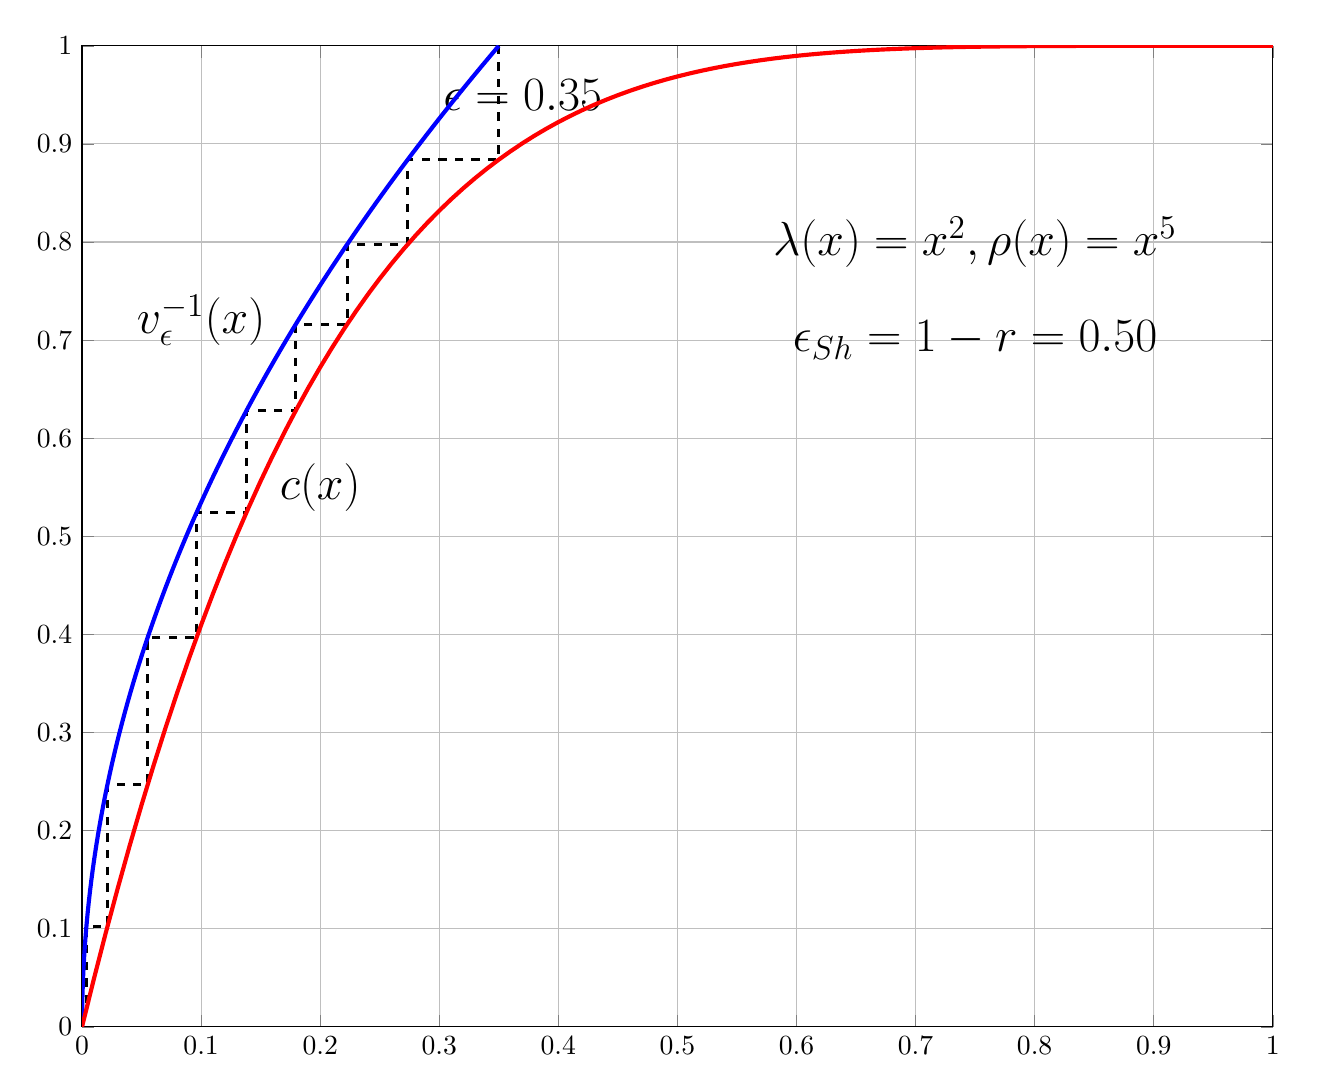
\begin{tikzpicture}
\def\fsize{\LARGE}
\begin{axis}[%
width=5.95380358705162in,
height=4.90490244969379in,
scale only axis,
xmin=0,
xmax=1,
xmajorgrids,
ymin=0,
ymax=1,
ymajorgrids
]
\node at (axis cs:0.2,0.55) {\fsize{$c(x)$}};
\node at (axis cs:0.1,0.72) {\fsize{$v_{\epsilon}^{-1}(x)$}};
\node at (axis cs:0.37,0.95) {\fsize{$\epsilon=0.35$}};

\node at (axis cs:0.75,0.8){\fsize{$\lambda(x)=x^2,\rho(x)=x^{5}$}};%\sum_{i=1}^{N}\binom{\alpha}{i}(-1)^{i-1}x^i$}};
\node at (axis cs:0.75,0.7){\fsize{$\epsilon_{\text{Sh}}=1-r=0.50 $}};
%\node at (axis cs:0.75,0.8){\fsize{$\rho(x)=x^{10},\alpha=0.1,N=50.$}};



\addplot [color=black,dashed,line width=1.0pt]
  table[row sep=crcr]{0.35	1\\
0.350000  0.883971 \\ 
0.273492  0.883971 \\ 
0.273492  0.797603 \\ 
0.222660  0.797603 \\ 
0.222660  0.716172 \\ 
0.179516  0.716172 \\ 
0.179516  0.628164 \\ 
0.138107  0.628164 \\ 
0.138107  0.524372 \\ 
0.096238  0.524372 \\ 
0.096238  0.397065 \\ 
0.055181  0.397065 \\ 
0.055181  0.247091 \\ 
0.021369  0.247091 \\ 
0.021369  0.102375 \\ 
0.003668  0.102375 \\ 
0.003668  0.018207 \\ 
0.000116  0.018207 \\ 
0.000116  0.000580 \\ 
0.000000  0.000580 \\ 
};
  
\addplot [color=blue,solid,line width=1.5pt]
  table[row sep=crcr]{0	0\\
3.5e-05	0.01\\
0.00014	0.02\\
0.000315	0.03\\
0.00056	0.04\\
0.000875	0.05\\
0.00126	0.06\\
0.001715	0.07\\
0.00224	0.08\\
0.002835	0.09\\
0.0035	0.1\\
0.004235	0.11\\
0.00504	0.12\\
0.005915	0.13\\
0.00686	0.14\\
0.007875	0.15\\
0.00896	0.16\\
0.010115	0.17\\
0.01134	0.18\\
0.012635	0.19\\
0.014	0.2\\
0.015435	0.21\\
0.01694	0.22\\
0.018515	0.23\\
0.02016	0.24\\
0.021875	0.25\\
0.02366	0.26\\
0.025515	0.27\\
0.02744	0.28\\
0.029435	0.29\\
0.0315	0.3\\
0.033635	0.31\\
0.03584	0.32\\
0.038115	0.33\\
0.04046	0.34\\
0.042875	0.35\\
0.04536	0.36\\
0.047915	0.37\\
0.05054	0.38\\
0.053235	0.39\\
0.056	0.4\\
0.058835	0.41\\
0.06174	0.42\\
0.064715	0.43\\
0.06776	0.44\\
0.070875	0.45\\
0.07406	0.46\\
0.077315	0.47\\
0.08064	0.48\\
0.084035	0.49\\
0.0875	0.5\\
0.091035	0.51\\
0.09464	0.52\\
0.098315	0.53\\
0.10206	0.54\\
0.105875	0.55\\
0.10976	0.56\\
0.113715	0.57\\
0.11774	0.58\\
0.121835	0.59\\
0.126	0.6\\
0.130235	0.61\\
0.13454	0.62\\
0.138915	0.63\\
0.14336	0.64\\
0.147875	0.65\\
0.15246	0.66\\
0.157115	0.67\\
0.16184	0.68\\
0.166635	0.69\\
0.1715	0.7\\
0.176435	0.71\\
0.18144	0.72\\
0.186515	0.73\\
0.19166	0.74\\
0.196875	0.75\\
0.20216	0.76\\
0.207515	0.77\\
0.21294	0.78\\
0.218435	0.79\\
0.224	0.8\\
0.229635	0.81\\
0.23534	0.82\\
0.241115	0.83\\
0.24696	0.84\\
0.252875	0.85\\
0.25886	0.86\\
0.264915	0.87\\
0.27104	0.88\\
0.277235	0.89\\
0.2835	0.9\\
0.289835	0.91\\
0.29624	0.92\\
0.302715	0.93\\
0.30926	0.94\\
0.315875	0.95\\
0.32256	0.96\\
0.329315	0.97\\
0.33614	0.98\\
0.343035	0.99\\
0.35	1\\
};
\addplot [color=red,solid,line width=1.5pt]
  table[row sep=crcr]{0	0\\
0.01	0.0490099501000001\\
0.02	0.0960792032000002\\
0.03	0.1412659743\\
0.04	0.1846273024\\
0.05	0.2262190625\\
0.06	0.2660959776\\
0.07	0.3043116307\\
0.08	0.3409184768\\
0.09	0.3759678549\\
0.1	0.40951\\
0.11	0.4415940551\\
0.12	0.4722680832\\
0.13	0.5015790793\\
0.14	0.5295729824\\
0.15	0.5562946875\\
0.16	0.5817880576\\
0.17	0.6060959357\\
0.18	0.6292601568\\
0.19	0.6513215599\\
0.2	0.67232\\
0.21	0.6922943601\\
0.22	0.7112825632\\
0.23	0.7293215843\\
0.24	0.7464474624\\
0.25	0.7626953125\\
0.26	0.7780993376\\
0.27	0.7926928407\\
0.28	0.8065082368\\
0.29	0.8195770649\\
0.3	0.83193\\
0.31	0.8435968651\\
0.32	0.8546066432\\
0.33	0.8649874893\\
0.34	0.8747667424\\
0.35	0.8839709375\\
0.36	0.8926258176\\
0.37	0.9007563457\\
0.38	0.9083867168\\
0.39	0.9155403699\\
0.4	0.92224\\
0.41	0.9285075701\\
0.42	0.9343643232\\
0.43	0.9398307943\\
0.44	0.9449268224\\
0.45	0.9496715625\\
0.46	0.9540834976\\
0.47	0.9581804507\\
0.48	0.9619795968\\
0.49	0.9654974749\\
0.5	0.96875\\
0.51	0.9717524751\\
0.52	0.9745196032\\
0.53	0.9770654993\\
0.54	0.9794037024\\
0.55	0.9815471875\\
0.56	0.9835083776\\
0.57	0.9852991557\\
0.58	0.9869308768\\
0.59	0.9884143799\\
0.6	0.98976\\
0.61	0.9909775801\\
0.62	0.9920764832\\
0.63	0.9930656043\\
0.64	0.9939533824\\
0.65	0.9947478125\\
0.66	0.9954564576\\
0.67	0.9960864607\\
0.68	0.9966445568\\
0.69	0.9971370849\\
0.7	0.99757\\
0.71	0.9979488851\\
0.72	0.9982789632\\
0.73	0.9985651093\\
0.74	0.9988118624\\
0.75	0.9990234375\\
0.76	0.9992037376\\
0.77	0.9993563657\\
0.78	0.9994846368\\
0.79	0.9995915899\\
0.8	0.99968\\
0.81	0.9997523901\\
0.82	0.9998110432\\
0.83	0.9998580143\\
0.84	0.9998951424\\
0.85	0.9999240625\\
0.86	0.9999462176\\
0.87	0.9999628707\\
0.88	0.9999751168\\
0.89	0.9999838949\\
0.9	0.99999\\
0.91	0.9999940951\\
0.92	0.9999967232\\
0.93	0.9999983193\\
0.94	0.9999992224\\
0.95	0.9999996875\\
0.96	0.9999998976\\
0.97	0.9999999757\\
0.98	0.9999999968\\
0.99	0.9999999999\\
1	1\\
};
\end{axis}
\end{tikzpicture}%}
\end{center}
\end{column}

\begin{column}{0.47\textwidth}
\begin{center}
\scalebox{0.35}{% This file was created by matlab2tikz v0.4.7 running on MATLAB 7.14.
% Copyright (c) 2008--2014, Nico Schlömer <nico.schloemer@gmail.com>
% All rights reserved.
% Minimal pgfplots version: 1.3
% 
% The latest updates can be retrieved from
%   http://www.mathworks.com/matlabcentral/fileexchange/22022-matlab2tikz
% where you can also make suggestions and rate matlab2tikz.
% 
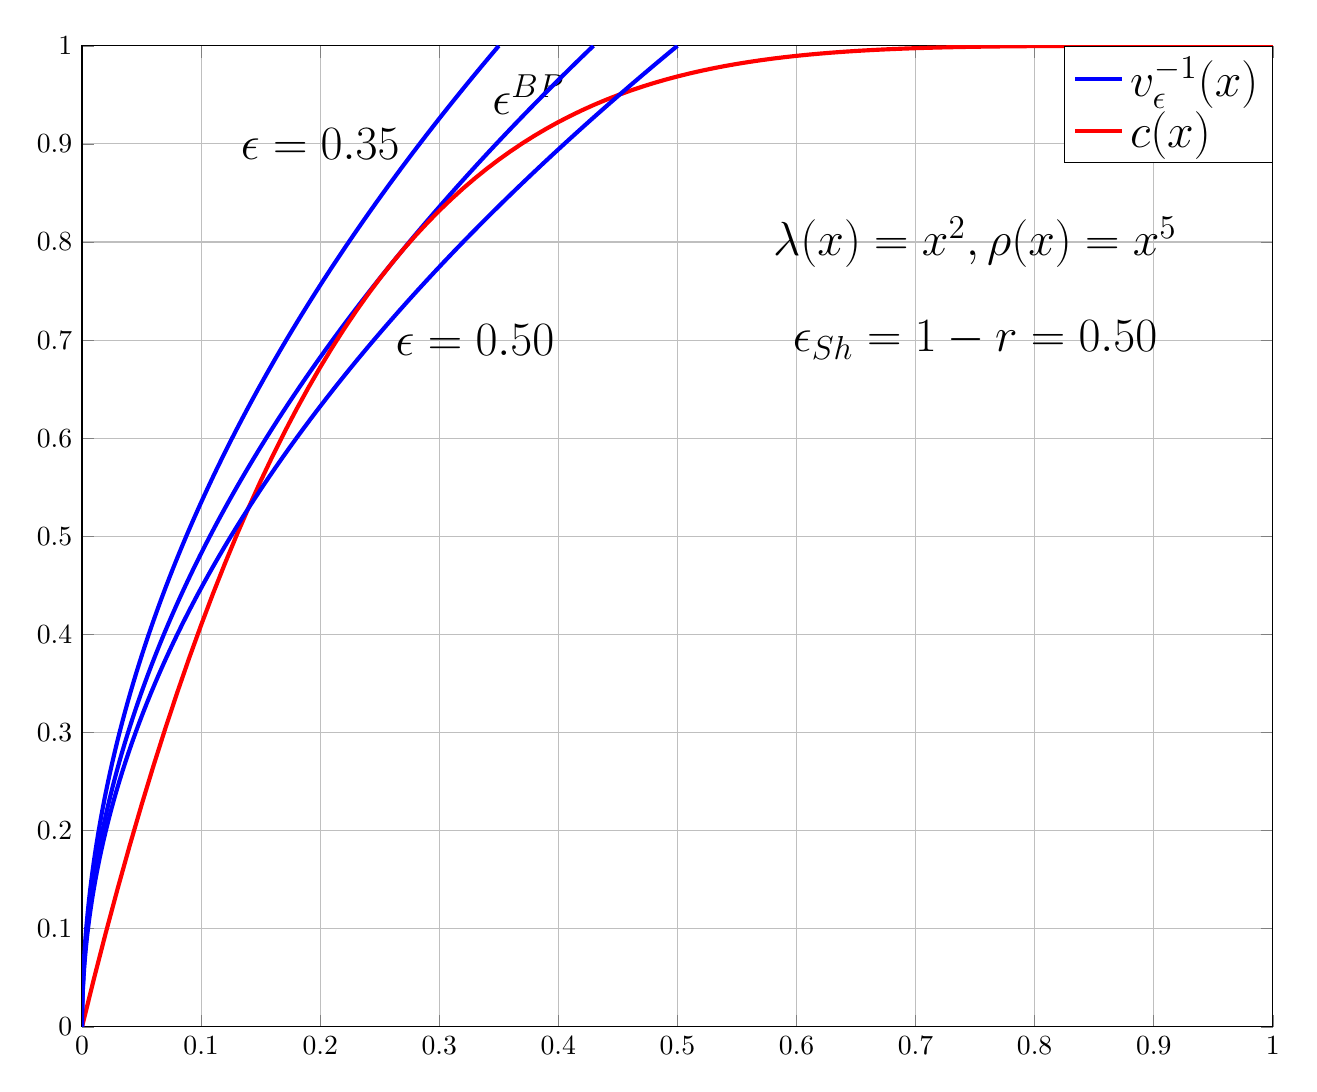
\begin{tikzpicture}
\def\fsize{\LARGE}
\begin{axis}[%
width=5.95380358705162in,
height=4.90490244969379in,
scale only axis,
xmin=0,
xmax=1,
xmajorgrids,
ymin=0,
ymax=1,
legend style={at={(1,1)},anchor=north east,draw=black,fill=white,legend cell align=left,font=\LARGE},
ymajorgrids
]
\node at (axis cs:0.33,0.7){\LARGE{$\epsilon=0.50$}};
\node at (axis cs:0.2,0.9){\LARGE{$\epsilon=0.35$}};
\node at (axis cs:0.375,0.95){\LARGE{$\epsilon^{\text{BP}}$}};

\node at (axis cs:0.75,0.8){\fsize{$\lambda(x)=x^2,\rho(x)=x^{5}$}};%\sum_{i=1}^{N}\binom{\alpha}{i}(-1)^{i-1}x^i$}};
\node at (axis cs:0.75,0.7){\fsize{$\epsilon_{\text{Sh}}=1-r=0.50 $}};

\addlegendentry{\LARGE{$v_{\epsilon}^{-1}(x)$}};
\addplot [color=blue,solid,line width=1.5pt]
  table[row sep=crcr]{0	0\\
4.2944e-05	0.01\\
0.000171776	0.02\\
0.000386496	0.03\\
0.000687104	0.04\\
0.0010736	0.05\\
0.001545984	0.06\\
0.002104256	0.07\\
0.002748416	0.08\\
0.003478464	0.09\\
0.0042944	0.1\\
0.005196224	0.11\\
0.006183936	0.12\\
0.007257536	0.13\\
0.008417024	0.14\\
0.0096624	0.15\\
0.010993664	0.16\\
0.012410816	0.17\\
0.013913856	0.18\\
0.015502784	0.19\\
0.0171776	0.2\\
0.018938304	0.21\\
0.020784896	0.22\\
0.022717376	0.23\\
0.024735744	0.24\\
0.02684	0.25\\
0.029030144	0.26\\
0.031306176	0.27\\
0.033668096	0.28\\
0.036115904	0.29\\
0.0386496	0.3\\
0.041269184	0.31\\
0.043974656	0.32\\
0.046766016	0.33\\
0.049643264	0.34\\
0.0526064	0.35\\
0.055655424	0.36\\
0.058790336	0.37\\
0.062011136	0.38\\
0.065317824	0.39\\
0.0687104	0.4\\
0.072188864	0.41\\
0.075753216	0.42\\
0.079403456	0.43\\
0.083139584	0.44\\
0.0869616	0.45\\
0.090869504	0.46\\
0.094863296	0.47\\
0.098942976	0.48\\
0.103108544	0.49\\
0.10736	0.5\\
0.111697344	0.51\\
0.116120576	0.52\\
0.120629696	0.53\\
0.125224704	0.54\\
0.1299056	0.55\\
0.134672384	0.56\\
0.139525056	0.57\\
0.144463616	0.58\\
0.149488064	0.59\\
0.1545984	0.6\\
0.159794624	0.61\\
0.165076736	0.62\\
0.170444736	0.63\\
0.175898624	0.64\\
0.1814384	0.65\\
0.187064064	0.66\\
0.192775616	0.67\\
0.198573056	0.68\\
0.204456384	0.69\\
0.2104256	0.7\\
0.216480704	0.71\\
0.222621696	0.72\\
0.228848576	0.73\\
0.235161344	0.74\\
0.24156	0.75\\
0.248044544	0.76\\
0.254614976	0.77\\
0.261271296	0.78\\
0.268013504	0.79\\
0.2748416	0.8\\
0.281755584	0.81\\
0.288755456	0.82\\
0.295841216	0.83\\
0.303012864	0.84\\
0.3102704	0.85\\
0.317613824	0.86\\
0.325043136	0.87\\
0.332558336	0.88\\
0.340159424	0.89\\
0.3478464	0.9\\
0.355619264	0.91\\
0.363478016	0.92\\
0.371422656	0.93\\
0.379453184	0.94\\
0.3875696	0.95\\
0.395771904	0.96\\
0.404060096	0.97\\
0.412434176	0.98\\
0.420894144	0.99\\
0.42944	1\\
};

\addlegendentry{\LARGE{$c(x)$}};
\addplot [color=red,solid,line width=1.5pt]
  table[row sep=crcr]{0	0\\
0.01	0.0490099501000001\\
0.02	0.0960792032000002\\
0.03	0.1412659743\\
0.04	0.1846273024\\
0.05	0.2262190625\\
0.06	0.2660959776\\
0.07	0.3043116307\\
0.08	0.3409184768\\
0.09	0.3759678549\\
0.1	0.40951\\
0.11	0.4415940551\\
0.12	0.4722680832\\
0.13	0.5015790793\\
0.14	0.5295729824\\
0.15	0.5562946875\\
0.16	0.5817880576\\
0.17	0.6060959357\\
0.18	0.6292601568\\
0.19	0.6513215599\\
0.2	0.67232\\
0.21	0.6922943601\\
0.22	0.7112825632\\
0.23	0.7293215843\\
0.24	0.7464474624\\
0.25	0.7626953125\\
0.26	0.7780993376\\
0.27	0.7926928407\\
0.28	0.8065082368\\
0.29	0.8195770649\\
0.3	0.83193\\
0.31	0.8435968651\\
0.32	0.8546066432\\
0.33	0.8649874893\\
0.34	0.8747667424\\
0.35	0.8839709375\\
0.36	0.8926258176\\
0.37	0.9007563457\\
0.38	0.9083867168\\
0.39	0.9155403699\\
0.4	0.92224\\
0.41	0.9285075701\\
0.42	0.9343643232\\
0.43	0.9398307943\\
0.44	0.9449268224\\
0.45	0.9496715625\\
0.46	0.9540834976\\
0.47	0.9581804507\\
0.48	0.9619795968\\
0.49	0.9654974749\\
0.5	0.96875\\
0.51	0.9717524751\\
0.52	0.9745196032\\
0.53	0.9770654993\\
0.54	0.9794037024\\
0.55	0.9815471875\\
0.56	0.9835083776\\
0.57	0.9852991557\\
0.58	0.9869308768\\
0.59	0.9884143799\\
0.6	0.98976\\
0.61	0.9909775801\\
0.62	0.9920764832\\
0.63	0.9930656043\\
0.64	0.9939533824\\
0.65	0.9947478125\\
0.66	0.9954564576\\
0.67	0.9960864607\\
0.68	0.9966445568\\
0.69	0.9971370849\\
0.7	0.99757\\
0.71	0.9979488851\\
0.72	0.9982789632\\
0.73	0.9985651093\\
0.74	0.9988118624\\
0.75	0.9990234375\\
0.76	0.9992037376\\
0.77	0.9993563657\\
0.78	0.9994846368\\
0.79	0.9995915899\\
0.8	0.99968\\
0.81	0.9997523901\\
0.82	0.9998110432\\
0.83	0.9998580143\\
0.84	0.9998951424\\
0.85	0.9999240625\\
0.86	0.9999462176\\
0.87	0.9999628707\\
0.88	0.9999751168\\
0.89	0.9999838949\\
0.9	0.99999\\
0.91	0.9999940951\\
0.92	0.9999967232\\
0.93	0.9999983193\\
0.94	0.9999992224\\
0.95	0.9999996875\\
0.96	0.9999998976\\
0.97	0.9999999757\\
0.98	0.9999999968\\
0.99	0.9999999999\\
1	1\\
};

\addplot [color=blue,solid,line width=1.5pt]
  table[row sep=crcr]{0	0\\
3.5e-05	0.01\\
0.00014	0.02\\
0.000315	0.03\\
0.00056	0.04\\
0.000875	0.05\\
0.00126	0.06\\
0.001715	0.07\\
0.00224	0.08\\
0.002835	0.09\\
0.0035	0.1\\
0.004235	0.11\\
0.00504	0.12\\
0.005915	0.13\\
0.00686	0.14\\
0.007875	0.15\\
0.00896	0.16\\
0.010115	0.17\\
0.01134	0.18\\
0.012635	0.19\\
0.014	0.2\\
0.015435	0.21\\
0.01694	0.22\\
0.018515	0.23\\
0.02016	0.24\\
0.021875	0.25\\
0.02366	0.26\\
0.025515	0.27\\
0.02744	0.28\\
0.029435	0.29\\
0.0315	0.3\\
0.033635	0.31\\
0.03584	0.32\\
0.038115	0.33\\
0.04046	0.34\\
0.042875	0.35\\
0.04536	0.36\\
0.047915	0.37\\
0.05054	0.38\\
0.053235	0.39\\
0.056	0.4\\
0.058835	0.41\\
0.06174	0.42\\
0.064715	0.43\\
0.06776	0.44\\
0.070875	0.45\\
0.07406	0.46\\
0.077315	0.47\\
0.08064	0.48\\
0.084035	0.49\\
0.0875	0.5\\
0.091035	0.51\\
0.09464	0.52\\
0.098315	0.53\\
0.10206	0.54\\
0.105875	0.55\\
0.10976	0.56\\
0.113715	0.57\\
0.11774	0.58\\
0.121835	0.59\\
0.126	0.6\\
0.130235	0.61\\
0.13454	0.62\\
0.138915	0.63\\
0.14336	0.64\\
0.147875	0.65\\
0.15246	0.66\\
0.157115	0.67\\
0.16184	0.68\\
0.166635	0.69\\
0.1715	0.7\\
0.176435	0.71\\
0.18144	0.72\\
0.186515	0.73\\
0.19166	0.74\\
0.196875	0.75\\
0.20216	0.76\\
0.207515	0.77\\
0.21294	0.78\\
0.218435	0.79\\
0.224	0.8\\
0.229635	0.81\\
0.23534	0.82\\
0.241115	0.83\\
0.24696	0.84\\
0.252875	0.85\\
0.25886	0.86\\
0.264915	0.87\\
0.27104	0.88\\
0.277235	0.89\\
0.2835	0.9\\
0.289835	0.91\\
0.29624	0.92\\
0.302715	0.93\\
0.30926	0.94\\
0.315875	0.95\\
0.32256	0.96\\
0.329315	0.97\\
0.33614	0.98\\
0.343035	0.99\\
0.35	1\\
};

\addplot [color=blue,solid,line width=1.5pt]
  table[row sep=crcr]{0	0\\
5e-05	0.01\\
0.0002	0.02\\
0.00045	0.03\\
0.0008	0.04\\
0.00125	0.05\\
0.0018	0.06\\
0.00245	0.07\\
0.0032	0.08\\
0.00405	0.09\\
0.005	0.1\\
0.00605	0.11\\
0.0072	0.12\\
0.00845	0.13\\
0.0098	0.14\\
0.01125	0.15\\
0.0128	0.16\\
0.01445	0.17\\
0.0162	0.18\\
0.01805	0.19\\
0.02	0.2\\
0.02205	0.21\\
0.0242	0.22\\
0.02645	0.23\\
0.0288	0.24\\
0.03125	0.25\\
0.0338	0.26\\
0.03645	0.27\\
0.0392	0.28\\
0.04205	0.29\\
0.045	0.3\\
0.04805	0.31\\
0.0512	0.32\\
0.05445	0.33\\
0.0578	0.34\\
0.06125	0.35\\
0.0648	0.36\\
0.06845	0.37\\
0.0722	0.38\\
0.07605	0.39\\
0.08	0.4\\
0.08405	0.41\\
0.0882	0.42\\
0.09245	0.43\\
0.0968	0.44\\
0.10125	0.45\\
0.1058	0.46\\
0.11045	0.47\\
0.1152	0.48\\
0.12005	0.49\\
0.125	0.5\\
0.13005	0.51\\
0.1352	0.52\\
0.14045	0.53\\
0.1458	0.54\\
0.15125	0.55\\
0.1568	0.56\\
0.16245	0.57\\
0.1682	0.58\\
0.17405	0.59\\
0.18	0.6\\
0.18605	0.61\\
0.1922	0.62\\
0.19845	0.63\\
0.2048	0.64\\
0.21125	0.65\\
0.2178	0.66\\
0.22445	0.67\\
0.2312	0.68\\
0.23805	0.69\\
0.245	0.7\\
0.25205	0.71\\
0.2592	0.72\\
0.26645	0.73\\
0.2738	0.74\\
0.28125	0.75\\
0.2888	0.76\\
0.29645	0.77\\
0.3042	0.78\\
0.31205	0.79\\
0.32	0.8\\
0.32805	0.81\\
0.3362	0.82\\
0.34445	0.83\\
0.3528	0.84\\
0.36125	0.85\\
0.3698	0.86\\
0.37845	0.87\\
0.3872	0.88\\
0.39605	0.89\\
0.405	0.9\\
0.41405	0.91\\
0.4232	0.92\\
0.43245	0.93\\
0.4418	0.94\\
0.45125	0.95\\
0.4608	0.96\\
0.47045	0.97\\
0.4802	0.98\\
0.49005	0.99\\
0.5	1\\
};
\end{axis}
\end{tikzpicture}%}
\end{center}

\end{column}

\end{columns}
\end{frame}
%--------------------------------------------------------------------------------------
\begin{frame}{Optimality of EXIT chart matching}
\begin{itemize}
\item Var node function: $v_{\epsilon}(x) = \epsilon \lambda(x)$
\item Check node function: $c(x) = 1- \rho(1-x)$
\end{itemize}
\begin{center}
\scalebox{0.45}{% This file was created by matlab2tikz v0.4.7 running on MATLAB 7.14.
% Copyright (c) 2008--2014, Nico Schlömer <nico.schloemer@gmail.com>
% All rights reserved.
% Minimal pgfplots version: 1.3
% 
% The latest updates can be retrieved from
%   http://www.mathworks.com/matlabcentral/fileexchange/22022-matlab2tikz
% where you can also make suggestions and rate matlab2tikz.
% 
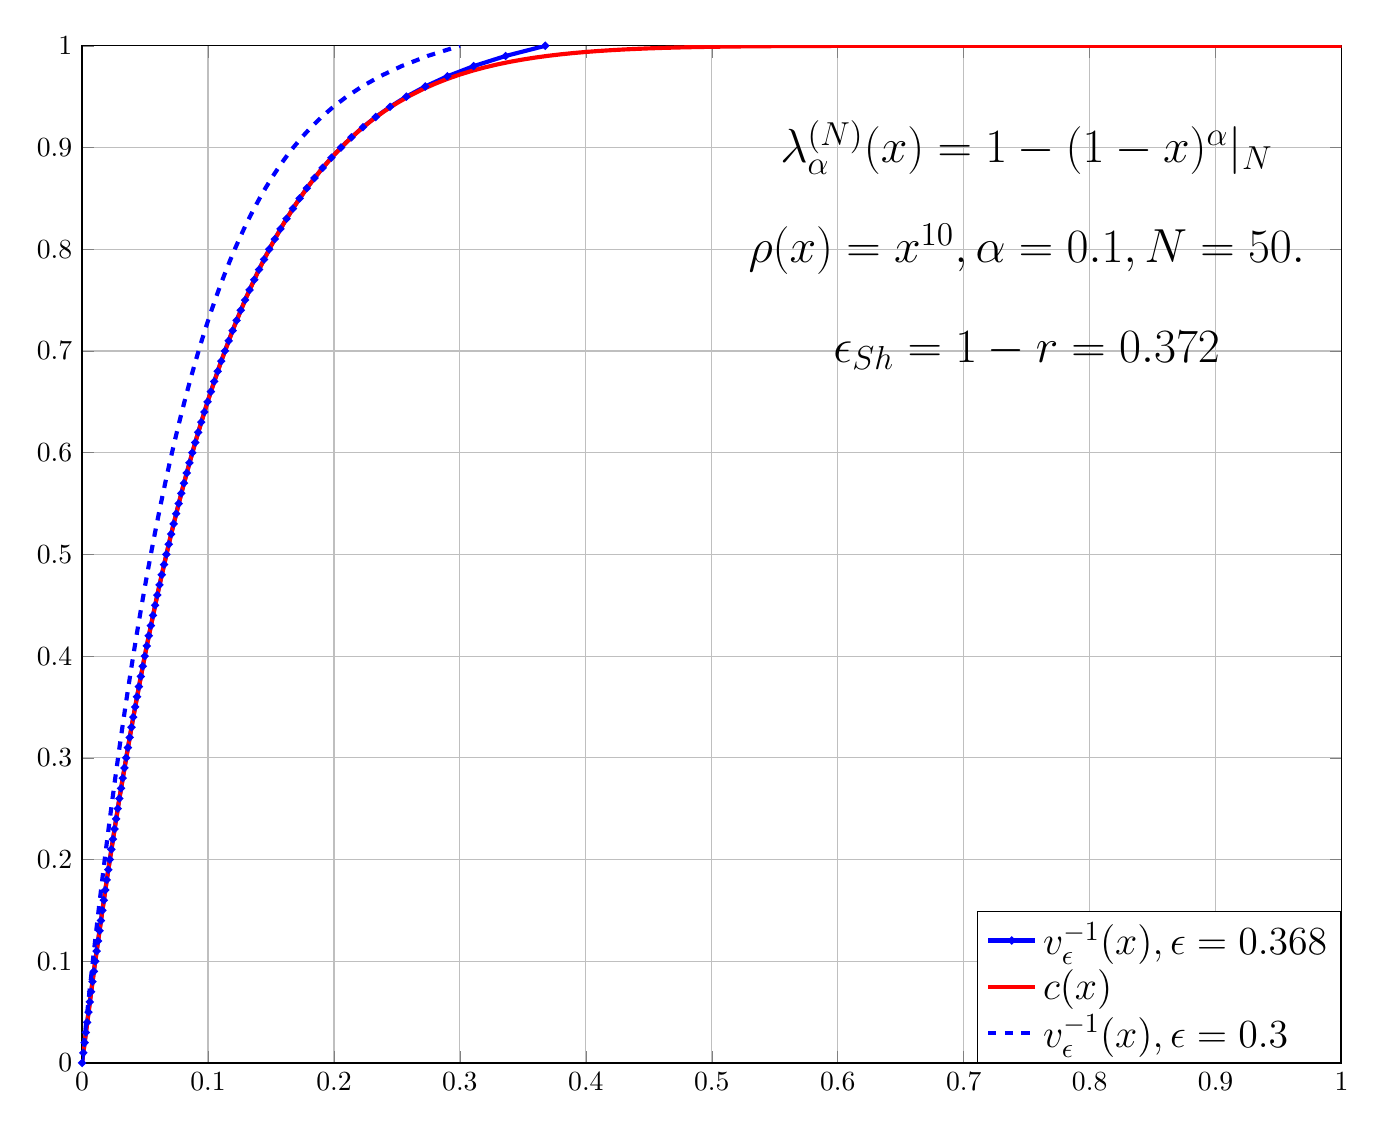
\begin{tikzpicture}
\def \fsize{\LARGE}
\begin{axis}[%
width=6.29770559930009in,
height=5.08572834645669in,
scale only axis,
xmin=0,
xmax=1,
xmajorgrids,
ymin=0,
ymax=1,
legend style={at={(1,0)},anchor=south east,draw=black,fill=white,legend cell align=left,font=\fsize},
ymajorgrids
]

\node at (axis cs:0.75,0.9){\fsize{$\lambda_{\alpha}^{(N)}(x)=1-(1-x)^{\alpha}|_{N}$}};%\sum_{i=1}^{N}\binom{\alpha}{i}(-1)^{i-1}x^i$}};
\node at (axis cs:0.75,0.8){\fsize{$\rho(x)=x^{10},\alpha=0.1,N=50.$}};
\node at (axis cs:0.75,0.7){\fsize{$\epsilon_{\text{Sh}}=1-r=0.372 $}};


\addlegendentry{\Large{$v_{\epsilon}^{-1}(x),\epsilon=0.368$}};
\addplot [color=blue,mark=*,mark size=0.5pt,solid,line width=1.5pt]
  table[row sep=crcr]{0	0\\
0.00100452870824995	0.01\\
0.00201823135843042	0.02\\
0.0030412866381062	0.03\\
0.00407387860214938	0.04\\
0.0051161968918237	0.05\\
0.00616843696522343	0.06\\
0.00723080033978309	0.07\\
0.00830349484762741	0.08\\
0.00938673490458918	0.09\\
0.0104807417937856	0.1\\
0.0115857439647124	0.11\\
0.0127019773488898	0.12\\
0.0138296856931755	0.13\\
0.0149691209119498	0.14\\
0.0161205434594737	0.15\\
0.0172842227238285	0.16\\
0.0184604374439603	0.17\\
0.0196494761514822	0.18\\
0.0208516376390232	0.19\\
0.0220672314570715	0.2\\
0.0232965784414229	0.21\\
0.0245400112735353	0.22\\
0.0257978750762919	0.23\\
0.0270705280479034	0.24\\
0.0283583421369265	0.25\\
0.0296617037616551	0.26\\
0.0309810145774423	0.27\\
0.0323166922958518	0.28\\
0.0336691715599149	0.29\\
0.0350389048801824	0.3\\
0.0364263636367327	0.31\\
0.0378320391528112	0.32\\
0.0392564438463597	0.33\\
0.040700112466341	0.34\\
0.0421636034214935	0.35\\
0.043647500209963	0.36\\
0.0451524129591818	0.37\\
0.046678980086392	0.38\\
0.0482278700913825	0.39\\
0.0497997834943236	0.4\\
0.0513954549330765	0.41\\
0.0530156554360524	0.42\\
0.0546611948886202	0.43\\
0.0563329247132606	0.44\\
0.0580317407861738	0.45\\
0.0597585866159188	0.46\\
0.0615144568129612	0.47\\
0.0633004008827987	0.48\\
0.0651175273797047	0.49\\
0.0669670084631926	0.5\\
0.0688500849051623	0.51\\
0.0707680716025138	0.52\\
0.0727223636579612	0.53\\
0.0747144431010848	0.54\\
0.0767458863325731	0.55\\
0.0788183723874597	0.56\\
0.0809336921283443	0.57\\
0.0830937584975923	0.58\\
0.0853006179789351	0.59\\
0.0875564634445046	0.6\\
0.0898636485940515	0.61\\
0.0922247042301274	0.62\\
0.0946423566578192	0.63\\
0.0971195485521326	0.64\\
0.0996594627027419	0.65\\
0.102265549127682	0.66\\
0.104941556148684	0.67\\
0.10769156614654	0.68\\
0.110520036871966	0.69\\
0.113431849385121	0.7\\
0.116432363947291	0.71\\
0.119527485507556	0.72\\
0.122723740837558	0.73\\
0.126028369898529	0.74\\
0.129449434717698	0.75\\
0.132995949962507	0.76\\
0.13667804060955	0.77\\
0.14050713372094	0.78\\
0.144496193519323	0.79\\
0.148660011914131	0.8\\
0.153015570690002	0.81\\
0.157582497173504	0.82\\
0.162383642994294	0.83\\
0.167445826487868	0.84\\
0.172800794707139	0.85\\
0.17848648289442	0.86\\
0.184548680493846	0.87\\
0.191043257563369	0.88\\
0.198039169928183	0.89\\
0.205622554612463	0.9\\
0.213902362190138	0.91\\
0.22301816904284	0.92\\
0.233151098427202	0.93\\
0.244539196204305	0.94\\
0.257499215745708	0.95\\
0.272457655587535	0.96\\
0.289995192326096	0.97\\
0.310910548784957	0.98\\
0.336312608378763	0.99\\
0.367753630095884	1\\
};
\addlegendentry{\Large{$c(x)$}};
\addplot [color=red,solid,line width=1.5pt]
  table[row sep=crcr]{0	0\\
0.01	0.0956179249911957\\
0.02	0.182927193112453\\
0.03	0.262575873105072\\
0.04	0.335167364008499\\
0.05	0.401263060761621\\
0.06	0.461384885905101\\
0.07	0.516017692820707\\
0.08	0.565611545776368\\
0.09	0.610583881881892\\
0.1	0.6513215599\\
0.11	0.688182800700338\\
0.12	0.721499023990598\\
0.13	0.751576585808564\\
0.14	0.778698421111969\\
0.15	0.803125595659277\\
0.16	0.825098771234019\\
0.17	0.844839588127942\\
0.18	0.862551968664039\\
0.19	0.878423345409431\\
0.2	0.8926258176\\
0.21	0.905317239173732\\
0.22	0.916642241687638\\
0.23	0.926733195274138\\
0.24	0.935711110676601\\
0.25	0.943686485290527\\
0.26	0.950760096026441\\
0.27	0.957023741702964\\
0.28	0.962560937573755\\
0.29	0.967447564489901\\
0.3	0.9717524751\\
0.31	0.975538059393452\\
0.32	0.978860771798428\\
0.33	0.981771621954482\\
0.34	0.984316631190892\\
0.35	0.986537256655371\\
0.36	0.988470784953931\\
0.37	0.990150697081182\\
0.38	0.991607006341317\\
0.39	0.992866570883371\\
0.4	0.9939533824\\
0.41	0.994888832466994\\
0.42	0.995691957931006\\
0.43	0.996379666685431\\
0.44	0.996966945109039\\
0.45	0.997467048378809\\
0.46	0.997891674807351\\
0.47	0.998251125296345\\
0.48	0.998554448940509\\
0.49	0.998809575761724\\
0.5	0.9990234375\\
0.51	0.999202077337024\\
0.52	0.999350749378915\\
0.53	0.999474008677642\\
0.54	0.999575792525172\\
0.55	0.99965949371084\\
0.56	0.999728026390616\\
0.57	0.999783885176867\\
0.58	0.999829198018783\\
0.59	0.999865773406899\\
0.6	0.9998951424\\
0.61	0.999918595939148\\
0.62	0.99993721788152\\
0.63	0.999951914156276\\
0.64	0.999963438415599\\
0.65	0.999972414526465\\
0.66	0.999979356222459\\
0.67	0.999984684210147\\
0.68	0.999988741000932\\
0.69	0.99999180371713\\
0.7	0.9999940951\\
0.71	0.999995792927667\\
0.72	0.999997038032333\\
0.73	0.999997941088679\\
0.74	0.999998588329043\\
0.75	0.999999046325684\\
0.76	0.99999936596619\\
0.77	0.999999585734888\\
0.78	0.999999734400772\\
0.79	0.99999983320119\\
0.8	0.9999998976\\
0.81	0.999999938689337\\
0.82	0.999999964295328\\
0.83	0.999999979840061\\
0.84	0.999999989004884\\
0.85	0.999999994233496\\
0.86	0.999999997107453\\
0.87	0.999999998621415\\
0.88	0.999999999380826\\
0.89	0.999999999740626\\
0.9	0.9999999999\\
0.91	0.999999999965132\\
0.92	0.999999999989263\\
0.93	0.999999999997175\\
0.94	0.999999999999395\\
0.95	0.999999999999902\\
0.96	0.99999999999999\\
0.97	0.999999999999999\\
0.98	1\\
0.99	1\\
1	1\\
};
\addlegendentry{\Large{$v_{\epsilon}^{-1}(x),\epsilon=0.3$}};
\addplot [color=blue,dashed,line width=1.5pt]
  table[row sep=crcr]{0	0\\
0.000819457886510628	0.01\\
0.00164639954028805	0.02\\
0.00248097072813115	0.03\\
0.00332332159529237	0.04\\
0.00417360684419873	0.05\\
0.00503198592243547	0.06\\
0.00589862322057662	0.07\\
0.00677368828049021	0.08\\
0.00765735601479321	0.09\\
0.00854980693818275	0.1\\
0.00945122741142626	0.11\\
0.0103618098988538	0.12\\
0.0112817532402628	0.13\\
0.0122112629382179	0.14\\
0.0131505514618066	0.15\\
0.0140998385680016	0.16\\
0.01505935164187	0.17\\
0.0160293260569792	0.18\\
0.0170100055574597	0.19\\
0.0180016426633107	0.2\\
0.0190044991006741	0.21\\
0.0200188462589508	0.22\\
0.021044965676803	0.23\\
0.0220831495592677	0.24\\
0.0231337013284133	0.25\\
0.0241969362101917	0.26\\
0.0252731818603922	0.27\\
0.0263627790328753	0.28\\
0.0274660822935749	0.29\\
0.0285834607840962	0.3\\
0.0297152990391164	0.31\\
0.0308619978622215	0.32\\
0.032023975265281	0.33\\
0.0332016674769976	0.34\\
0.0343955300268553	0.35\\
0.0356060389113626	0.36\\
0.036833691850228	0.37\\
0.0380790096409556	0.38\\
0.039342537621294	0.39\\
0.0406248472500511	0.4\\
0.041926537818003	0.41\\
0.0432482383020092	0.42\\
0.0445906093770183	0.43\\
0.0459543456024401	0.44\\
0.0473401778014074	0.45\\
0.0487488756537941	0.46\\
0.0501812505265462	0.47\\
0.0516381585679748	0.48\\
0.0531205040962288	0.49\\
0.0546292433162922	0.5\\
0.056165388404632	0.51\\
0.0577300120061867	0.52\\
0.0593242521948733	0.53\\
0.0609493179563758	0.54\\
0.0626064952608869	0.55\\
0.0642971538039552	0.56\\
0.0660227545059794	0.57\\
0.0677848578755788	0.58\\
0.0695851333595495	0.59\\
0.0714253698230057	0.6\\
0.0733074873283682	0.61\\
0.075233550412064	0.62\\
0.0772057830943585	0.63\\
0.0792265859022063	0.64\\
0.0812985552393523	0.65\\
0.0834245055046918	0.66\\
0.085607494442398	0.67\\
0.0878508523098423	0.68\\
0.0901582155774912	0.69\\
0.092533566036218	0.7\\
0.0949812763916973	0.71\\
0.0975061636860457	0.72\\
0.100113552221546	0.73\\
0.102809348094541	0.74\\
0.105600128012833	0.75\\
0.108493245813371	0.76\\
0.111496961082816	0.77\\
0.114620595601713	0.78\\
0.117874725110108	0.79\\
0.12127141630828	0.8\\
0.124824522316835	0.81\\
0.128550054393006	0.82\\
0.132466654062903	0.83\\
0.136596198746599	0.84\\
0.140964586532091	0.85\\
0.145602763606616	0.86\\
0.150548083328827	0.87\\
0.155846122454502	0.88\\
0.161553132631116	0.89\\
0.167739381301703	0.9\\
0.174493746371206	0.91\\
0.181930089161616	0.92\\
0.190196163420396	0.93\\
0.199486158279835	0.94\\
0.210058469588923	0.95\\
0.222261019299658	0.96\\
0.236567502202889	0.97\\
0.253629487249842	0.98\\
0.274351561090839	0.99\\
0.3	1\\
};
\end{axis}
\end{tikzpicture}%}
\end{center}
\end{frame}
%%------------------------------------------------------------------------------------
%\begin{frame}{Low density generator matrix (LDGM) codes}
%\vspace{-3mm}
%\begin{columns}
%\begin{column}{0.47\textwidth}
%\begin{center}
%\includegraphics[width=2.0in]{LDGMoverbec}
%\end{center}
%\end{column}
%\begin{column}{0.47\textwidth}
%\begin{itemize}
%\item $L(x) = \frac14 x + \frac14 x^2 + \frac12 x^3$
%\vspace{2mm}
%\item $\lambda(x) = \frac19 + \frac29 x + \frac 69 x^2$
%\vspace{2mm}
%\item $R(x) = \frac15 x + \frac45 x^2$
%\vspace{2mm}
%\item $\rho(x) = \frac19 + \frac89 x$
%\vspace{2mm}
%\item Rate $R = \frac{\int_{0}^{1}\lambda(x) \ dx}{\int_{0}^{1} \rho(x) \ dx}$
%\end{itemize}
%\end{column}
%\end{columns}
%
%\begin{columns}
%\column{0.45\textwidth}
%\begin{block}{DE for LDPC}
%\vspace*{-3mm}
%\begin{eqnarray*}
%  x_0 &=& \epsilon \\
%  y_l &=& 1-\rho(1-x_{l-1}) \\
%  x_l &=& \epsilon \lambda(y_l)\\
%  x_l &=& \epsilon \lambda(1-\rho(1-x_{l-1}))
%\end{eqnarray*}
%\end{block}
%
%\column{0.45\textwidth}
%\begin{block}{DE for LDGM}
%\vspace*{-3mm}
%\begin{eqnarray*}
%  x_0 &=& 1 \\
%  y_l &=& 1-(1-\epsilon) \rho(1-x_{l-1}) \\
%  x_l &=& \lambda(y_l) \\
%  x_l &=& \lambda(1-(1-\epsilon)\rho(1-x_{l-1}))
%\end{eqnarray*}
%\end{block}
%\end{columns}
%\end{frame}
%%-------------------------------------------------------------------------------------
%\begin{frame}{What are rateless codes?}
%\begin{center}
%  \includegraphics[width=3.5in]{ratelesssystem}
%\end{center}
%\begin{block}{Multicast with different channel qualities}
%\begin{itemize}
%\item Code should be simultaneously optimal for all $\epsilon$
%\item Want to create potentially endless stream of coded bits
%\end{itemize}
%\end{block}
%\pause
%\begin{block}{Downloading from multiple servers}
%\begin{itemize}
%\item Do not want to download the same coded bit multiple times
%\item Randomized encoding strategy is beneficial
%\end{itemize}
%\end{block}
%\end{frame}
%%--------------------------------------------------------------------------------------
%\begin{frame}{LDGM codes and rateless codes}
%\begin{center}
%  \includegraphics[width=2.75in]{ratelesserasures1}
%\end{center}
%
%\begin{block}{LT Codes, Luby'02}
%\begin{itemize}
%  \item Choose the degree according to a distribution $f_D$
%  \item Pick bits uniformly at random to make linear combination
%  \item Left degree is Poisson : $\lambda(x) = e^{-r_{avg}(1-x)}$
%\end{itemize}
%\end{block}
%\end{frame}
%%--------------------------------------------------------------------------------------
%\begin{frame}{Poisson, soliton pair is optimal for rateless codes}
%\vspace{-3mm}
%\begin{columns}
%\column{0.55\textwidth}
%\begin{center}
%\scalebox{0.45}{% This file was created by matlab2tikz v0.4.7 running on MATLAB 7.14.
% Copyright (c) 2008--2014, Nico Schlömer <nico.schloemer@gmail.com>
% All rights reserved.
% Minimal pgfplots version: 1.3
% 
% The latest updates can be retrieved from
%   http://www.mathworks.com/matlabcentral/fileexchange/22022-matlab2tikz
% where you can also make suggestions and rate matlab2tikz.
% 
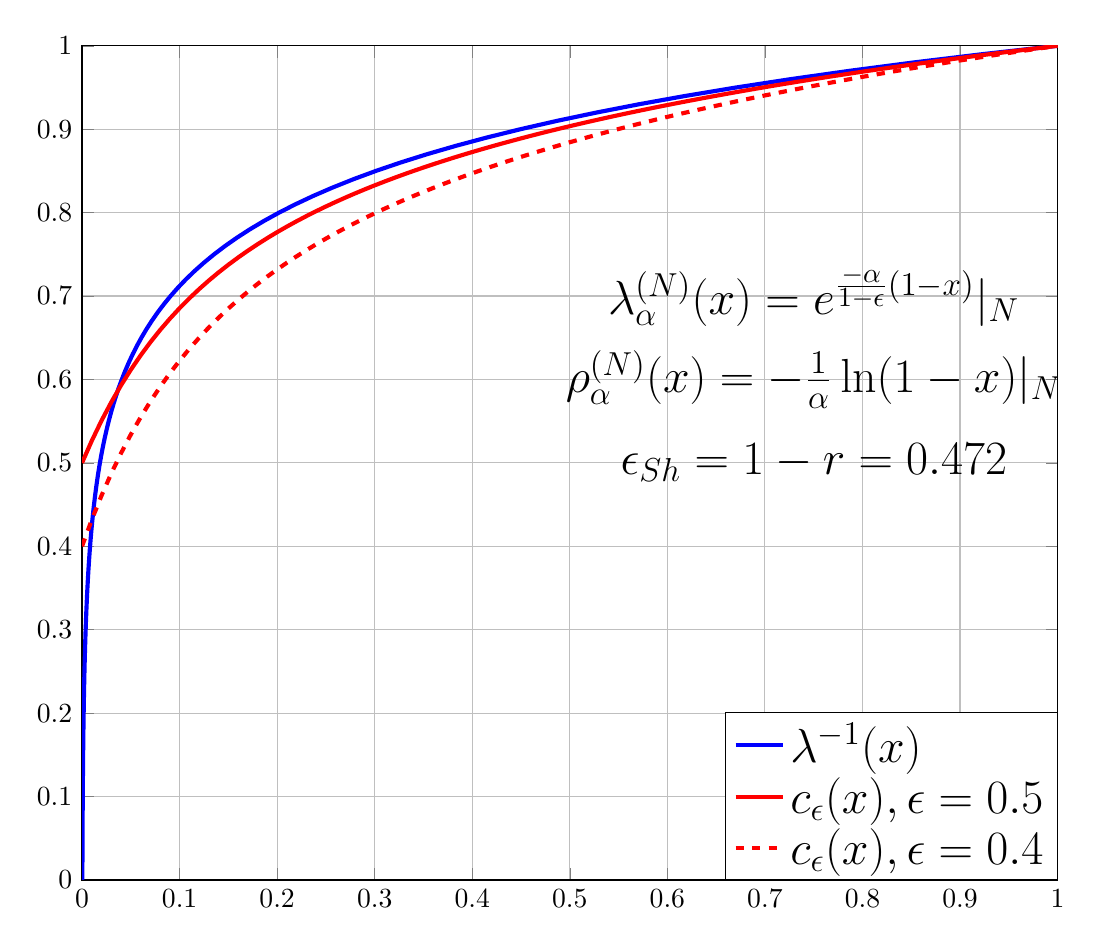
\begin{tikzpicture}
\def\fsize{\LARGE}

\begin{axis}[%
width=4.87804024496938in,
height=4.17068372703412in,
scale only axis,
xmin=0,
xmax=1,
xmajorgrids,
xtick={0,0.1,0.2,...,1},
xticklabels={0,0.1,0.2,0.3,0.4,0.5,0.6,0.7,0.8,0.9,1},
ymin=0,
ymax=1,
legend style={at={(1,0)},anchor=south east,draw=black,fill=white,legend cell align=left,font=\LARGE},
ymajorgrids
]
\node at (axis cs:0.75,0.7){\fsize{$\lambda_{\alpha}^{(N)}(x)=e^{\frac{-\alpha}{1-\epsilon} (1-x)}|_{N}$}};
%\sum\limits_{i=1}^{N}\frac{1}{\alpha}\frac{x^i}{i}}};
\node at (axis cs:0.75,0.6){\fsize{$\rho_{\alpha}^{(N)}(x)=-\frac{1}{\alpha}\ln (1-x)|_{N}$}};
%x^{\frac{1}{\alpha}},\alpha=0.1,N=50$}};
\node at (axis cs:0.75,0.5){\fsize{$\epsilon_{\text{Sh}}=1-r=0.472$}};

\addlegendentry{$\lambda^{-1}(x)$};
\addplot [color=blue,solid,line width=1.5pt]
  table[row sep=crcr]{0.000335494153584825	0\\
0.000363436477858997	0.01\\
0.000393706036385988	0.02\\
0.000426496657682508	0.03\\
0.000462018313674054	0.04\\
0.000500498464232096	0.05\\
0.000542183513693807	0.06\\
0.00058734038869107	0.07\\
0.000636258247392219	0.08\\
0.000689250331101526	0.09\\
0.000746655970072966	0.1\\
0.000808842756382345	0.11\\
0.000876208897771561	0.12\\
0.000949185767537662	0.13\\
0.00102824066679468	0.14\\
0.00111387981679615	0.15\\
0.00120665160047942	0.16\\
0.00130715007398865	0.17\\
0.00141601877066227	0.18\\
0.00153395482184343	0.19\\
0.00166171342090063	0.2\\
0.00180011265904357	0.21\\
0.00195003876389988	0.22\\
0.0021124517743976	0.23\\
0.00228839168829194	0.24\\
0.00247898512170151	0.25\\
0.00268545252329786	0.26\\
0.00290911598934362	0.27\\
0.00315140772962231	0.28\\
0.00341387923847058	0.29\\
0.00369821122963888	0.3\\
0.00400622439859745	0.31\\
0.00433989108120327	0.32\\
0.00470134788338308	0.33\\
0.00509290936270569	0.34\\
0.00551708284945217	0.35\\
0.00597658450208934	0.36\\
0.00647435669995645	0.37\\
0.00701358688453719	0.38\\
0.00759772796996556	0.39\\
0.00823052045346203	0.4\\
0.00891601636728181	0.41\\
0.00965860522554881	0.42\\
0.0104630421321226	0.43\\
0.0113344782294832	0.44\\
0.0122784936836085	0.45\\
0.0133011334160577	0.46\\
0.0144089458120634	0.47\\
0.0156090246524914	0.48\\
0.0169090545381691	0.49\\
0.0183173600974417	0.5\\
0.0198429592920402	0.51\\
0.0214956211625829	0.52\\
0.0232859283834527	0.53\\
0.0252253450275842	0.54\\
0.0273262899750436	0.55\\
0.0296022164354101	0.56\\
0.0320676980931018	0.57\\
0.0347385224271733	0.58\\
0.0376317918030286	0.59\\
0.0407660329832215	0.6\\
0.0441613157583836	0.61\\
0.0478393814576613	0.62\\
0.0518237821612379	0.63\\
0.0561400315059548	0.64\\
0.060815768049174	0.65\\
0.0658809322363014	0.66\\
0.0713679581043317	0.67\\
0.0773119809479292	0.68\\
0.0837510622765184	0.69\\
0.0907264335012647	0.7\\
0.098282759910384	0.71\\
0.106468426620664	0.72\\
0.115335848333247	0.73\\
0.124941804873458	0.74\\
0.135347804658769	0.75\\
0.146620478416798	0.76\\
0.15883200566779	0.77\\
0.172060576694392	0.78\\
0.186390892947055	0.79\\
0.201914709077521	0.8\\
0.218731420056951	0.81\\
0.23694869712112	0.82\\
0.256683176594334	0.83\\
0.278061205978336	0.84\\
0.301219652054399	0.85\\
0.326306776138336	0.86\\
0.353483182051611	0.87\\
0.382922842829663	0.88\\
0.41481421268376	0.89\\
0.449361431268097	0.9\\
0.486785627882633	0.91\\
0.527326333867846	0.92\\
0.571243012123746	0.93\\
0.618816713416241	0.94\\
0.670351869923472	0.95\\
0.726178237327734	0.96\\
0.786652997679963	0.97\\
0.852163036258837	0.98\\
0.923127406721123	0.99\\
1	1\\
};

\addlegendentry{$c_{\epsilon}(x),\epsilon=0.5$};
\addplot [color=red,solid,line width=1.5pt]
  table[row sep=crcr]{0	0.5\\
0.01	0.526526126042806\\
0.02	0.550706243040251\\
0.03	0.57280262188789\\
0.04	0.593046195873519\\
0.05	0.6116403489369\\
0.06	0.628764252863599\\
0.07	0.644575805441883\\
0.08	0.659214215869252\\
0.09	0.672802278552915\\
0.1	0.685448371847462\\
0.11	0.697248214159826\\
0.12	0.708286406177705\\
0.13	0.718637784699063\\
0.14	0.728368610616949\\
0.15	0.73753761100972\\
0.16	0.746196892968877\\
0.17	0.754392744735548\\
0.18	0.762166337885451\\
0.19	0.769554342676617\\
0.2	0.776589467232609\\
0.21	0.783300929956643\\
0.22	0.789714873441285\\
0.23	0.795854727138328\\
0.24	0.801741525169708\\
0.25	0.807394184880162\\
0.26	0.812829751044085\\
0.27	0.818063610032608\\
0.28	0.82310967771285\\
0.29	0.827980564381521\\
0.3	0.832687719622072\\
0.31	0.837241559611941\\
0.32	0.841651579088144\\
0.33	0.84592644990045\\
0.34	0.850074107836845\\
0.35	0.854101829192009\\
0.36	0.858016298362217\\
0.37	0.861823667586471\\
0.38	0.865529609810601\\
0.39	0.869139365526266\\
0.4	0.87265778432787\\
0.41	0.876089361835362\\
0.42	0.879438272548156\\
0.43	0.882708399123219\\
0.44	0.885903358507587\\
0.45	0.889026525300862\\
0.46	0.892081052675632\\
0.47	0.89506989114236\\
0.48	0.897995805409208\\
0.49	0.900861389555933\\
0.5	0.903669080713676\\
0.51	0.906421171418762\\
0.52	0.909119820787906\\
0.53	0.911767064644275\\
0.54	0.914364824708154\\
0.55	0.91691491695232\\
0.56	0.919419059210307\\
0.57	0.921878878115366\\
0.58	0.924295915438839\\
0.59	0.926671633888754\\
0.6	0.929007422422485\\
0.61	0.931304601121274\\
0.62	0.93356442566907\\
0.63	0.935788091473473\\
0.64	0.937976737462459\\
0.65	0.94013144958696\\
0.66	0.94225326405617\\
0.67	0.944343170329661\\
0.68	0.946402113887892\\
0.69	0.948430998800506\\
0.7	0.950430690109856\\
0.71	0.952402016045493\\
0.72	0.954345770083781\\
0.73	0.95626271286546\\
0.74	0.958153573982763\\
0.75	0.960019053646566\\
0.76	0.961859824243142\\
0.77	0.963676531789142\\
0.78	0.965469797292704\\
0.79	0.967240218027864\\
0.8	0.968988368728802\\
0.81	0.970714802709912\\
0.82	0.972420052917143\\
0.83	0.974104632915626\\
0.84	0.97576903781815\\
0.85	0.977413745158703\\
0.86	0.979039215714913\\
0.87	0.980645894282958\\
0.88	0.982234210408185\\
0.89	0.983804579074453\\
0.9	0.985357401354956\\
0.91	0.986893065027096\\
0.92	0.988411945153746\\
0.93	0.989914404633095\\
0.94	0.991400794719091\\
0.95	0.992871455514339\\
0.96	0.994326716437194\\
0.97	0.995766896664656\\
0.98	0.997192305552543\\
0.99	0.998603243034339\\
1	1\\
};

\addlegendentry{$c_{\epsilon}(x),\epsilon=0.4$};
\addplot [color=red,dashed,line width=1.5pt]
  table[row sep=crcr]{0	0.4\\
0.01	0.431831351251367\\
0.02	0.460847491648301\\
0.03	0.487363146265468\\
0.04	0.511655435048223\\
0.05	0.533968418724279\\
0.06	0.554517103436319\\
0.07	0.57349096653026\\
0.08	0.591057059043103\\
0.09	0.607362734263498\\
0.1	0.622538046216955\\
0.11	0.63669785699179\\
0.12	0.649943687413245\\
0.13	0.662365341638875\\
0.14	0.674042332740338\\
0.15	0.685045133211665\\
0.16	0.695436271562653\\
0.17	0.705271293682658\\
0.18	0.714599605462541\\
0.19	0.723465211211941\\
0.2	0.731907360679131\\
0.21	0.739961115947971\\
0.22	0.747657848129542\\
0.23	0.755025672565993\\
0.24	0.76208983020365\\
0.25	0.768873021856194\\
0.26	0.775395701252902\\
0.27	0.781676332039129\\
0.28	0.78773161325542\\
0.29	0.793576677257825\\
0.3	0.799225263546487\\
0.31	0.804689871534329\\
0.32	0.809981894905773\\
0.33	0.81511173988054\\
0.34	0.820088929404215\\
0.35	0.82492219503041\\
0.36	0.82961955803466\\
0.37	0.834188401103766\\
0.38	0.838635531772721\\
0.39	0.84296723863152\\
0.4	0.847189341193444\\
0.41	0.851307234202435\\
0.42	0.855325927057787\\
0.43	0.859250078947862\\
0.44	0.863084030209105\\
0.45	0.866831830361034\\
0.46	0.870497263210758\\
0.47	0.874083869370832\\
0.48	0.87759496649105\\
0.49	0.881033667467119\\
0.5	0.884402896856411\\
0.51	0.887705405702515\\
0.52	0.890943784945487\\
0.53	0.89412047757313\\
0.54	0.897237789649784\\
0.55	0.900297900342784\\
0.56	0.903302871052369\\
0.57	0.906254653738439\\
0.58	0.909155098526607\\
0.59	0.912005960666505\\
0.6	0.914808906906982\\
0.61	0.917565521345529\\
0.62	0.920277310802884\\
0.63	0.922945709768168\\
0.64	0.925572084954951\\
0.65	0.928157739504352\\
0.66	0.930703916867404\\
0.67	0.933211804395593\\
0.68	0.935682536665471\\
0.69	0.938117198560607\\
0.7	0.940516828131827\\
0.71	0.942882419254591\\
0.72	0.945214924100537\\
0.73	0.947515255438552\\
0.74	0.949784288779315\\
0.75	0.952022864375879\\
0.76	0.954231789091771\\
0.77	0.95641183814697\\
0.78	0.958563756751245\\
0.79	0.960688261633437\\
0.8	0.962786042474563\\
0.81	0.964857763251894\\
0.82	0.966904063500572\\
0.83	0.968925559498751\\
0.84	0.970922845381781\\
0.85	0.972896494190444\\
0.86	0.974847058857895\\
0.87	0.976775073139549\\
0.88	0.978681052489822\\
0.89	0.980565494889343\\
0.9	0.982428881625947\\
0.91	0.984271678032515\\
0.92	0.986094334184495\\
0.93	0.987897285559714\\
0.94	0.98968095366291\\
0.95	0.991445746617207\\
0.96	0.993192059724633\\
0.97	0.994920275997587\\
0.98	0.996630766663051\\
0.99	0.998323891641207\\
1	1\\
};
\end{axis}
\end{tikzpicture}}
%  %\includegraphics[width=2.2in]{EXIT_PoissSoliton}
%\end{center}
%\column{0.45\textwidth}
%\begin{center}
%  \includegraphics[width=2.2in]{ratelesserasures3}
%\end{center}
%\end{columns}
%%\begin{block}{Poisson, Soliton pair is optimal - $\lambda(x) = e^{-r_{avg}(1-x)}$}
%\begin{itemize}
%%\item Poisson, soliton pair is optimal
%  %\item Left degree is Poisson : $\lambda(x) = e^{-r_{avg}(1-x)}$
%  \item   $x = \lambda(1-(1-\epsilon)\rho(1-x))$
%  \item $\lambda(x) = e^{-\frac{\alpha}{1-\epsilon}(1-x)}$, \alert{optimal right degree is soliton: $\rho(x) = -\frac{1}{\alpha}\ln(1-x)$}
%  %\item \alert{Optimal distribution is soliton: $f_D[i] = \frac{1}{i(i-1)}$}
%\end{itemize}
%\begin{center}
%\begin{tabular}{|l|c|c|c|c|c|c|c|c|}
%\hline
%Degree of nodes & 1 & 2 & 3 & 4 & $\ldots$ & $i$ & \ldots & $K$ \\
%\hline
%Fraction: \alert{ $f_D[i]$ } & $\frac{1}{K}$ & $\frac12$ & $\frac16$ & $\frac{1}{12}$ & $\ldots$ & $\frac{1}{i(i-1)}$ & \ldots & $\frac{1}{K (K-1)}$ \\
%\hline
%\end{tabular}
%\end{center}
%%\end{block}
%\end{frame}
%%--------------------------------------------------------------------------------------
%\begin{frame}{Histogram of required $N$ for $K=10000$}
%\begin{center}
%  \includegraphics[width=4.2in]{fountaincodes10000histogram}
%\end{center}
%\begin{block}{Finite length considerations}
%\begin{itemize}
%  \item Deg. dist. must be adjusted for optimizing finite length performance
%  \item Raptor codes (Shokrollahi'06) is an excellent choice
%\end{itemize}
%\end{block}
%\end{frame}

%---------------------------------------------------------------------------------------
%\begin{frame}\frametitle{Questions?}
%	\begin{figure}[t]
%		\centering
%		\includegraphics[width=2.8in]{questions}
%	\end{figure}
%	\centering
%	\color{blue}
%	%\Huge{Thank you!}
%\end{frame}
%---------------------------------------------------------------------------------------
\begin{frame}{Summary}
\begin{itemize}
  \item Understand what degree distributions $(\lambda(x),\rho(x))$ mean
\pause
  \item Given a $(\lambda,\rho)$ and $\epsilon$, what will be the $P_e^n$ as $l,n \rightarrow \infty$ ?
\pause
  \item Can you compute the threshold?
\pause
  \item Is a $(\lambda(x),\rho(x))$ pair optimal?
\end{itemize}
\end{frame} 